% ProjectTemplate.tex LaTeX template for Complexity and Networks projects
% T.S.Evans, K. Christensen Imperial College, London

\documentclass[a4paper,12pt]{article}

\newcommand{\reporttitle}{Gaussian process regression methods for option pricing}
\newcommand{\reportauthor}{Nicholas Delmotte}
\newcommand{\supervisor}{Josef Teichmann}
\newcommand{\degreetype}{Master's degree in physics}

% The packages are useful for many mathematical symbols but you may well not need them
%\usepackage{amsmath,amssymb,amscd}

% This is great for reading in images
% \usepackage[draft]{graphicx}
\usepackage{graphicx}
\usepackage{float}
\usepackage{amsmath}
\usepackage{multicol}
\usepackage{subcaption}
\usepackage{hyperref}
\usepackage[ruled,vlined]{algorithm2e}
\usepackage{wrapfig}
\usepackage{enumitem}
\usepackage[final]{pdfpages}
\usepackage{makecell}
\usepackage{tabularx}
\usepackage{cite}
\usepackage{amsfonts}
\usepackage{bbold}
\usepackage{amsthm}


% This is great for drafts as it will show all the labels you have defined.
% DON'T forget to comment it out before submission
%\usepackage{showkeys}

% Change Page Size
\typeout{--- Increasing width and height of text }
% A4 paper is 297mm high and 210mm wide.
\setlength{\textwidth}{16.00cm} % OK for both Letter and A4
\setlength{\oddsidemargin}{-0.04cm}  % actual margins = 1inch + \oddsidemargin
                                 %top/odd/even-sidemargin
\setlength{\evensidemargin}{-0.04cm} %  ditto
\setlength{\topmargin}{-1.0cm}      %  ditto
\setlength{\headheight}{18pt} \setlength{\headsep}{6pt}
\setlength{\topskip}{0pt}  %see pp155 also about baselineskip
\setlength{\textheight}{25.0cm} % 25cm for A4, 23cm for Letter or DJ
\setlength{\footskip}{0.7cm}




\begin{document}

% Last modification: 2015-08-17 (Marc Deisenroth)
\begin{titlepage}

\newcommand{\HRule}{\rule{\linewidth}{0.5mm}} % Defines a new command for the horizontal lines, change thickness here


%----------------------------------------------------------------------------------------
%	LOGO SECTION
%----------------------------------------------------------------------------------------

\hspace*{-1.6cm}
\includegraphics[width = 6cm]{eth_logo.png}\\[0.5cm] 

\center % Center remainder of the page

%----------------------------------------------------------------------------------------
%	HEADING SECTIONS
%----------------------------------------------------------------------------------------

\textsc{\Large Eidgenössische Technische Hochschule Zürich}\\[0.5cm] 
\textsc{\large Department of Mathematics}\\[0.5cm] 

%----------------------------------------------------------------------------------------
%	TITLE SECTION
%----------------------------------------------------------------------------------------

\HRule \\[0.4cm]
{ \huge \bfseries \reporttitle}\\ % Title of your document
\HRule \\[1.5cm]
 
%----------------------------------------------------------------------------------------
%	AUTHOR SECTION
%----------------------------------------------------------------------------------------

\begin{minipage}{0.4\textwidth}
\begin{flushleft} \large
\emph{Author:}\\
\reportauthor % Your name
\end{flushleft}
\end{minipage}
~
\begin{minipage}{0.4\textwidth}
\begin{flushright} \large
\emph{Supervisor:} \\
\supervisor % Supervisor's Name
\end{flushright}
\end{minipage}\\[4cm]


%----------------------------------------------------------------------------------------
%	FOOTER & DATE SECTION
%----------------------------------------------------------------------------------------
\vfill % Fill the rest of the page with whitespace

\makeatletter
\@date 
\makeatother


\end{titlepage}


\pagenumbering{roman}
\setcounter{page}{1}

\vspace*{\fill}
\begin{center}
    \large
    \textbf{Abstract}
\end{center}
This thesis presents the theory of Gaussian process regression and applies it to an option pricing context. Specifically, this technique is first used to price call options using as input variables the strike price $K$ and the time-to-maturity $T$ of the option; the option price is then derived to obtain Greeks. It is shown that, when setting appropriate prior conditions on some hyperparameters of the model and when choosing a proper training data set, the Greek estimates are very accurate. In a second stage, the Gaussian process model is adapted to price any input European payoff function. This model performs well compared to the finite element method, but shows some limitations when applied to market data. Applying No Arbitrage conditions on the model is also shown to improve its estimates by half an order of magnitude in the mean squared error. Finally, in a third stage, the model is adapted again to price American and European options simultaneously. This model is shown to perform better than two independent models that price these options separately.

\vspace*{\fill}

\newpage

\section*{Acknowledgments}
I would first like to acknowledge my colleague Daniel Montagna who worked with me during the first few weeks of the thesis. Much of the first part of this thesis was the fruit of a collaborative effort between us. As such, there may exist some similarities between the introduction of Gaussian process theory in his thesis \cite{Montagna2021} and my own.\\
I would also like to thank my supervisors: Wahid, Jakob, Hanna, and Philippe. Their weekly input helped guide and shape much of the innovations presented in this thesis.\\
Finally, I would like to thank my supervising professor, Josef Teichmann, for allowing me to complete my Master thesis in his group and for offering several pointed and pertinent comments about the validity of certain Gaussian process assumptions (some of which are featured in this thesis).


\newpage
\setcounter{tocdepth}{2}
\tableofcontents

\newpage

\pagenumbering{arabic}
\setcounter{page}{1}

\section{Introduction}
The idea of using Gaussian processes for prediction finds its roots in the field of geostatistics. It was Matheron \cite{Matheron1963} who first formalised the concept and popularised the term `kriging' as a method of interpolation for predicting the grade of a mining panel. His work was based on the Master thesis of Krige \cite{Krige2015}, the term's eponym, although the basic theory can be traced back to Wiener's \cite{Wiener1949} and Kolmogorov's \cite{Kolmogorov1941} works in time series analysis in the 1940s. Kriging was originally formulated as a linear predictor but it has since evolved and become more synonymous with Gaussian process regression, and has been adopted by many other fields: hydrology \cite{Zimmerman1998}, weather prediction \cite{Karnieli1990}, astronomy \cite{Pastorello2014}, aircraft design \cite{Chung2002}.\\
Wiliams and Rasmussen \cite{Williams1996} introduced Gaussian process regression to the world of machine learning, and detailed algorithms for training the hyperparameters of the covariance function, also called the kernel. In fact, the efficient training of these hyperparameters is one of the many strengths of this interpolation method. Another point of comparison is that standard interpolation methods such as splines yield worse results for non-uniform knots, which isn't necessarily the case with Gaussian processes. It is also very advantageous that the Bayesian structure of Gaussian process regression yields not only point estimates but also the uncertainty of the predictions at those points, a feature which is not shared by frequentist techniques such as neural networks.\\
The adoption of Gaussian processes in a financial setting is much more recent than in the aforementioned fields. Some examples include the use of kriging for credit scoring \cite{Fernandes2016}, valuation of Bermudan options \cite{ludkovski2016}, optimizing financial asset portfolios \cite{Barrosa2016}, and financial derivative modeling \cite{Cousin2016}. This last application constitutes the focus of this thesis, which covers various uses of Gaussian processes in relation to option pricing. In fact, this thesis is divided into three parts.\\
The first introduces the theory behind Gaussian process regression and follows the work of Ludkovski and Saporito \cite{Ludkovski2020} that takes option pricing one step further and derives a Gaussian process to obtain Greeks. This thesis replicates Ludkovski and Saporito's model (which was implemented in R) in Python using the \texttt{Tensorflow} package, and takes advantage of its automatic differentiation feature to augment said model.\\
The second part of the thesis explores the use of a functional Gaussian process, that is to say a Gaussian process that takes a function as an input, in order to price any European option. The idea is similar to that of the finite element method, wherein a set of basis (training) functions are used to interpolate any random European payoff (test) function.\\
The last part of the thesis investigates how multi-output Gaussian processes can be used to improve estimates of European and American option prices. Here the idea is to create a model which generates two outputs (European option price and American option price) for any given input, whereas standard Gaussian processes only have one output. The intention behind multi-output learning is that the correlation between the outputs will improve the performance of the model compared to several models learning the separate outputs independently. Such a model should therefore yield more accurate option prices than those yielded by a standard Gaussian process, as described in the first part of the thesis.\\
By exploring these various uses of kriging, this thesis attempts to establish a strong foundational understanding of the implementation and training of Gaussian processes (particularly in Python), and the common challenges that one is likely to face when attempting to replicate the methods presented herein. Additionally, this thesis proposes some novel perspectives that can hopefully underline the unique potential of these methods in improving option price estimates, or even in pricing completely original options.


\section{An in-depth look into option pricing and Greek estimation using Gaussian process regression \label{sec:ludkovski}}
This first part of the thesis follows the paper \cite{Ludkovski2020} titled `KrigHedge: Gaussian Process Surrogates for Delta Hedging' by Ludkovski and Saporito. It serves as an introduction to the ideas and algorithms behind Gaussian process regression, and presents a Python implementation \footnote{The Python code used for each part of this thesis can be found at \url{https://github.com/nicdel-git/master_thesis}.} of those algorithms.

\subsection{A brief overview of some financial concepts}
\subsubsection{Delta hedging}
In a very general sense, options in finance are contracts that reward the contract holder with a positive payoff depending on the performance of a certain underlying, which in this thesis will always be a stock. The two most common options are calls and puts (resp.) which convey their holder the right to buy or sell (resp.) the underlying stock for a predetermined strike price on a predetermined maturity date. A call option holder is rewarded if the underlying stock does well, and a put option holder is rewarded if it does poorly.\\
The Delta of an option is simply its partial derivative with respect to the value of its underlying: $\Delta = \frac{\partial V}{\partial S}$, where $V$ is the value of the option and $S$ is the value of its underlying. The efficient computation of this Delta is the main interest of the paper \cite{Ludkovski2020}. The reason this quantity is of particular interest is that Delta represents the sensitivity of the option payoff (which is equal to its price) to a change in the underlying stock price. Thus, one can buy or sell an amount of the stock that corresponds to the Delta of the option to create a delta neutral portfolio. In this case, the fluctuations in price of the stock and the option offset each other; the risk in the position is minimised. However, it should be noted that the movement of the stock and the option is only hedged at a single point in time, and so maintaining Delta neutrality requires dynamic hedging, i.e. continual re-investments in time. This is why it is also interesting to look at other Greeks like Theta and Gamma, as shown in the paper \cite{Ludkovski2020}.

\subsubsection{Different pricing models}
In 1973 \cite{Black1973}, \textbf{Black and Scholes} introduced a model for the evolution of stock prices:
\begin{equation}
\label{BS}
    dS = \mu S dt + \sigma S dW
\end{equation}
where $S$ is the stock price, $\mu$ is the drift, $\sigma$ is a constant volatility, and $W$ is a Brownian motion.\\
Equation \ref{BS} leads to an analytical expression for pricing European call options (i.e. options with only one exercise date, as opposed to American options which can be exercised at any time). However, one can also start with a market price for a call option and invert the pricing formula to obtain an ``implied volatility", i.e. the volatility implied by the market price. The Black-Scholes (B-S) model assumes this implied volatility is the same for all options, but market data actually suggests that implied volatilities change depending on the strike price and the time-to-maturity of the option. This phenomenon is called the volatility smile.\\
This means it is no longer possible to price all options with the same constant volatility. Moreover, it is no longer clear whether it is possible to hedge one option with another if they have different implied volatilities.\\
\newline
The \textbf{local volatility model}, introduced by Dupire \cite{Dupire1994} and Derman and Kani \cite{Derman1994}, solves these problems by adding a time and stock price dependency to the local volatility:
\begin{equation}
    dS = \mu S dt + \sigma(S,t) S dW
\end{equation}
In his paper \cite{Dupire1994}, Dupire states that ``knowledge of the prices of all path-dependent options is equivalent to knowledge of the full risk neutral diffusion process of the spot". This allows him to introduce a new way to price options using his local volatility model. This model is self-consistent, arbitrage-free and can be calibrated to match observed market smiles.\\
However, Hagan et al. \cite{Hagan2002} underline that the local volatility model prediction for the dynamic behaviour of smiles is opposite to market observations. This can lead to instability in delta and vega hedges, and makes the local volatility model a bad estimator of certain exotic options.\\
\newline
Hagan et al. thus introduce the SABR model \cite{Hagan2002}, which is a \textbf{stochastic volatility model}, to better describe the dynamics of the volatility smile. In a stochastic volatility model, the volatility itself is also governed by a Brownian motion:
\begin{align}
    dS &= \mu S dt + \sqrt{\nu} S dW_1\\
    d\nu &= \alpha dt + \beta dW_2 \\
    dW_1 dW_2 &= \rho dt
\end{align}
where $\nu$ is the variance of $S$, and $W_1$ and $W_2$ are two brownian motions correlated by $\rho$.\\
Stochastic volatility models capture more realistic dynamics of the volatility smile, and yield stable hedges. However, they are also harder to calibrate and raise some issues with the completeness of the market.\\
\newline
The paper \cite{Ludkovski2020} uses the Black-Scholes model and the local volatility model to generate simulated data to train and test a Gaussian Process method for computing Greeks. In this case, rather than using the market prices to compute an implied volatility, the paper establishes a set expression for the volatility and then uses the corresponding models to compute estimated market prices. In the Black-Scholes case this can be done analytically, but in the local volatility case it requires the use of Monte Carlo techniques.

\subsubsection{Option pricing and Greek computation in the Black-Scholes model}
Since both the paper by Ludkovski and Saporito and the vast majority of this thesis use Black-Scholes option prices as data for the models, it is of interest to write the formulae that allow the efficient computation of those prices. The Black-Scholes call option pricing formula was first derived in 1973 by Fischer Black and Myron Scholes \cite{Black1973}. There are many different possible proofs of the formula, and they are all well documented, so they won't be reproduced here. The formula is written thus:
\begin{equation}
\begin{gathered}
    C(K,T) = N(d_1) S_t + N(d_2) K e^{-r T} \\
    \text{where} \quad d_1 = \frac{\ln{\frac{S_t}{K}} + (r + \sigma^2)T}{\sigma \sqrt{T}} \quad \text{and} \quad d_2 = d_1 - \sigma \sqrt{T}
\end{gathered}
\end{equation}
Here, $S_t$ is the current price of the underlying, $K$ the strike price, $r$ the risk free rate, $T$ the time-to-maturity, $\sigma$ the volatility of the underlying, and $N$ the standard normal cumulative distribution function.\\
The pricing formula for put options can be obtained directly from the call price, using the put-call parity equation:
\begin{equation}
    C(K, T) - P(K, T) = S_t - e^{-r T}K
\end{equation}
The paper is concerned not only with the computation of call prices, but also with the computation of its associated Greeks (specifically Delta, Theta, and Gamma). These can also be obtained directly from the call price formula (the proofs aren't reproduced here but can easily be found elsewhere):
\begin{equation}
\begin{aligned}
    \Delta &= \frac{\partial C}{\partial S_t} = N(d_1)\\
    \Theta &= \frac{\partial C}{\partial t} = -\frac{S_t \sigma N'(d_1)}{2 \sqrt{T}} - r K e^{-r T} N(d_2)\\
    \Gamma &= \frac{\partial^2 C}{\partial S_t^2} = \frac{N'(d_1)}{S_t \sigma \sqrt{T}}
\end{aligned}
\end{equation}
Note that $N'(d_1) = \frac{1}{2\sqrt{\pi}} e^{-d_1^2/2}$.\\
Using the formulae above, we can obtain Black-Scholes prices with little computational cost. The prices are exact (for the B-S model), or in other words they are noiseless. For some cases it will be interesting to use noisy data instead. To obtain noisy prices, instead of using the exact formulae, it is possible to run a Monte Carlo simulation on the underlying stock prices. The idea is to start with $S_t$ and iterate over equation \ref{BS} for small time steps until we obtain the final price $S_T$ at the exercise date. We do this $N$ times to obtain a whole array of different final prices $S^i_T$, then we compute the mean payoff value $\frac{1}{N} \sum_{i = 1}^N |S^i_T - K|_+$. This mean value is the noisy call price $C(K, T)$, and it is more or less noisy depending on how big or small $N$ is. If $N$ were taken to infinity, we would obtain identical prices to those in the formulae above.

\subsection{Gaussian processes}
Armed with the basic concepts of financial derivative pricing, we can now turn towards the use of Gaussian processes for the estimation of these option prices. Indeed, whilst we have seen that option prices for the Black-Scholes model can be computed exactly, this is not true for the more complex (and more financially accurate) models. Nonetheless, even for those latter models it is possible to compute price estimates using Monte Carlo techniques. The motivation, then, for using Gaussian process regression for option pricing is that it is faster than Monte Carlo techniques, and that such processes can be trained directly with real financial data.
\subsubsection{Definition}
A Gaussian Process (GP) is a set of random variables ${X_t}$, $t$ in the index set $T$, such that any finite subset of these random variables follows a multivariate normal distribution. This is equivalent to saying that any finite linear combination of the random variables follows a 1-dimensional normal law. We can write:

$$(X_{t_1},\dots,X_{t_n}) \sim \mathcal{N}(\boldsymbol{\mu},\Sigma)$$
$$\boldsymbol{\mu} = \text{mean vector}, \quad \Sigma = \text{covariance matrix}$$
A covariance matrix, or kernel, is symmetric, positive semi-definite. In fact, conversely, any symmetric, positive semi-definite function can be taken as the covariance of a Gaussian process \cite{durrande}. This is useful since it means kernels can be added together, multiplied together, and composed with a function, and will still yield a kernel.

\subsubsection{Gaussian process regression}
Ludkovski and Saporito \cite{Ludkovski2020} suggest using Gaussian process regression, or kriging, to learn the pricing functional $\hat{P}$, then analytically derive the result to obtain the desired Greeks (Delta, Theta, Gamma). The map $\hat{P}$ is thus referred to as the surrogate.\\
Given a data set $\mathcal{D} = \{(t_i,S_i,Y_i) \}_{i=1}^N$ , we learn the pricing map $\hat{P}$ that approximates the option prices $Y_i$:
$$(t,S) \mapsto \hat{P}(t,S)$$
Then we compute the partial derivate of the estimate $\hat{P}$:
$$
\widehat{\Delta} = \frac{\partial \hat{P}}{\partial S}, \quad \widehat{\Theta} = \frac{\partial \hat{P}}{\partial t}
$$
The true structure of our data set is such that for each tuple $\mathbf{x}_i = (t_i,S_{t_i})$ we have a noisy price observation $Y_i \simeq P(t_i,S_{t_i})$, where $P(\cdot)$ is the `true' price. We then try to learn the price surface $\hat{P}(\mathbf{x})$ based on a Gaussian noise observation model.
$$ 
Y(\mathbf{x}) = P(\mathbf{x}) + \epsilon, \quad \epsilon \sim \mathcal{N}(0,\sigma^2_{\epsilon}) 
$$
We make the Gaussian process regression (GPR) assumption that the map $\mathbf{x}\mapsto P(\mathbf{x})$ is a realisation of a Gaussian random field, such that any subset $\{P(\mathbf{x}),\mathbf{x}\in \mathcal{X}\}$ is a multivariate Gaussian.
$$    
(P(\mathbf{x}_1),\dots,P(\mathbf{x}_n)) \sim \mathcal{N}(\mathbf{m}^n,K^{n \times n}) 
$$
For $n$ data points we identify the prior mean vector $\mathbf{m}^n$ and covariance matrix $K^{n \times n}$ as
$$ 
\mathbf{m}^n = (m(\mathbf{x}_1;\boldsymbol{\beta}), \dots,m(\mathbf{x}_n;\boldsymbol{\beta})), \quad
K^{n\times n}_{i,j} = \kappa(\mathbf{x}_i,\mathbf{x}_j;\boldsymbol{\beta})
$$
Here $\kappa(\cdot,\cdot)$ denotes a symmetric, positive semi-definite kernel function, and $\boldsymbol{\beta}$ is the vector of all hyperparameters.\\
Note that this GPR assumption is problematic from an economic perspective. Indeed, by assuming that the pricing function is Gaussian, we also admit that there is a non-zero probability that said price can be negative, which is of course impossible for options. An alternative we could pursue would be to pull the Gaussian random field into the noise term $\epsilon(\mathbf{x})$. This would yield an equivalent model but avoid the problem of assuming potentially negative `true' prices. Nevertheless, since Ludkovski and Saporito adopted the model described above, we shall also continue using it.\\
The aim of GPR is to estimate the posterior distribution of $P(\cdot)$ given the observation data $\mathcal{D}$ and assuming a Gaussian noise model. One observes that the conditional posterior predictive distribution $P(\mathbf{x}_*)| \{\mathbf{x}_i,y_i\}_{i=1}^n$ is also Gaussian, and its mean yields the GPR estimation of the price $\hat{P}(\mathbf{x}_*)$. We define this pointwise mean as $m_*$:
\begin{equation}
\label{eq:mean}
\begin{aligned}
  m_*(\mathbf{x}_*) &= \mathbb{E}[P(\mathbf{x}_*)|\mathbf{X},\mathbf{y}]\\
                    &= m(\mathbf{x_*}) + \mathbf{K}^T(K^{n\times n}+\sigma^2_{\epsilon}\mathbf{I})^{-1}(\mathbf{y}-\mathbf{m}^n)
\end{aligned}
\end{equation}
In the above equation we identify $\mathbf{x}_*$ as an abitrary input, $\mathbf{X} = [\mathbf{x}_1,\dots,\mathbf{x}_n]^T$ and $\mathbf{K}^T = [\kappa(\mathbf{x}_*,\mathbf{x}_1;\boldsymbol{\beta}),\dots,\kappa(\mathbf{x}_*\mathbf{x}_n;\boldsymbol{\beta})]$. Finally, the covariance of the posterior distribution on a chosen set of inputs $\{ \mathbf{x}_{*,i}\}_{i=1}^M$ is given by:
\begin{equation}
    \label{eq:covariance}
    (K_*)_{i,j} \equiv \text{Cov}(P(\mathbf{x}_{*,i}),P(\mathbf{x}_{*,j}))= \kappa(\mathbf{x}_{*,i},\mathbf{x}_{*,j};\boldsymbol{\beta})-\mathbf{K}_i^T(K^{n \times n}+\sigma^2_{\epsilon}\mathbf{I})^{-1}\mathbf{K}_j
\end{equation}
These two quantities provide the two key ingredients to our GPR approach: $m_*(\mathbf{x}_*)$ is the most likely estimate of $P(\mathbf{x}_*)$, whereas $\text{Var}(P(\mathbf{x}_*))$ indicates the model uncertainty at this point. 

\subsubsection{Optimisation by maximum likelihood estimation}
Gaussian Process Regression relies on determining appropriate values for the hyperparameters $\boldsymbol{\beta}$ that shape the posterior distribution. We find these hyperparameters in the prior kernel function, the prior mean function and the noise estimate (also known as the `nugget'). 
\begin{itemize}
    \item Kernel function: common choices include Gaussian (RBF) or Matérn ($5/2$, 3/2)
    $$ \kappa_{RBF}(\mathbf{x},\mathbf{x}')  = \sigma^2_p \exp{\left (-\sum_{k=1}^d\frac{(\mathbf{x}_k-\mathbf{x}'_k)^2}{2l_{\text{len},k}^2}\right )}$$
    $$
    \kappa_{M52}(\mathbf{x},\mathbf{x}') =\sigma_p^2 \prod_{k=1}^d \left(1+\frac{\sqrt{5}}{l_{\text{len},k}}|\mathbf{x}_k-\mathbf{x}'_k| +\frac{5}{3l^2_{\text{len},k}}(\mathbf{x}_k-\mathbf{x}'_k)^2 \right)e^{-\frac{\sqrt{5}}{l_{\text{len},k}}|\mathbf{x}_k-\mathbf{x}'_k|}
    $$
    Note that this definition of the Matérn kernel is the one given in the paper \cite{Ludkovski2020} by Ludkovski and Saporito. This definition differs from the one most commonly used in other papers and in the Python packages used in this thesis.\\
    \item Mean function: constant, linear, or polynomial 
    $$ m(\mathbf{x};\boldsymbol{\beta}) = \sum_{k=1}^K \beta_k\phi(\mathbf{x}), \quad \phi(\cdot) \text{ a polynomial basis} $$\\
    \item Observation noise: $$\epsilon \sim \mathcal{N}(0,\sigma^2_{\epsilon}) $$
\end{itemize}
The total set of hyperparameters to be trained is thus:
$$  \{\{\beta_i \}_{i=1}^K, \sigma^2_p,\{l_{\text{len},k} \}_{k=1}^d ,\sigma^2_{\epsilon}\} $$
Maximum likelihood estimation is used to find the optimal parameters for the model. The likelihood function of the parameters $\mathbf{\beta}$ given the data $\mathbf{y}$ is given by the multivariate Gaussian probability distribution $f(\mathbf{y} | \beta, \mathbf{x})$:
\begin{align*}
    \mathcal{L}(\beta | \mathbf{y}) &= f(\mathbf{y} | \beta, \mathbf{x})\\
    &= \frac{1}{2 \pi \sqrt{|K^{n \times n} + \sigma_\epsilon^2 \mathbb{1}|}} \exp [-\frac{1}{2}(\mathbf{y} - \mathbf{m}^n)^T(K^{n \times n} + \sigma_\epsilon^2 \mathbb{1})^{-1}(\mathbf{y} - \mathbf{m}^n)]
\end{align*}
The optimal hyperparameters $\mathbf{\beta}^\star$ are then found by the optimisation problem:
\begin{equation}
    \mathbf{\beta}^\star = \underset{\beta}{\arg\max} \mathcal{L}(\beta | \mathbf{y}) = \underset{\beta}{\arg\max} f(\mathbf{y} | \beta, \mathbf{x})
\end{equation}
Many algorithms will choose to minimise the negative log likelihood instead of maximising the likelihood. Both methods are equivalent.

\subsubsection{Approach for Greek estimation}
Having computed the posterior estimate of the option price $P(\mathbf{x}_*)$ and its uncertainty $\text{Var}(P(\mathbf{x}_*))$, as well as having established an algorithm for training the hyperparameters, we can now turn our attention to obtaining the Greeks using our surrogate model. Given our fitted GP model for the option price $GP(m_*,K_*)$, its derivative is again a GP model $GP(g_*,K_g)$. The mean function and covariance of the derivative GP are simply obtained by differentiation: 
\begin{equation}
\label{eq:greek_estimate}
\begin{aligned}
   g_{*,j}(\mathbf{x}_*) &= \frac{\partial m_*}{\partial x_j} (\mathbf{x}_*) = \frac{\partial m}{\partial x_j} (\mathbf{x}_*) + \frac{\partial \kappa}{\partial x_j}(\mathbf{x}_*,\mathbf{x})(K^{n \times n}+\sigma^2_{\epsilon}\textbf{I})^{-1}(\mathbf{y}-\mathbf{m}^n)\\
   K_g(\mathbf{x}_*,\mathbf{x}'_*) &= \frac{\partial^2 \kappa_*}{\partial x_j \partial x'_j}(\mathbf{x_*}, \mathbf{x'_*}) = \frac{\partial^2 \kappa}{\partial x_j \partial x_j'}(\mathbf{x_*}, \mathbf{x'_*}) - \frac{\partial \kappa}{\partial x_j}(\mathbf{x_*}, \mathbf{x})(K + \sigma_\epsilon^2 \mathbb{1})^{-1}\frac{\partial \kappa}{\partial x_j}(\mathbf{x}, \mathbf{x'_*})
\end{aligned}
\end{equation}
where $\mathbf{x_\star}$ and $\mathbf{x'_\star}$ represent test data, and $\mathbf{x}$ represents training data.\\
We can then identify:
$$
    \widehat{\Delta}(\mathbf{x}_*) = g_{*,S}(\mathbf{x}_*) \qquad \widehat{\Theta}(\mathbf{x}_*) = g_{*,t}(\mathbf{x}_*)
$$
In the paper \cite{Ludkovski2020} the Greek Gamma is also derived, using a finite differences method.\\
Defining $V_g(\mathbf{x}_*) =K_g(\mathbf{x}_*,\mathbf{x}_*)$, the confidence bounds are given by:
$$
CI_{\alpha} = \left [g_{*}(\mathbf{x}_*) - z_{\alpha}\sqrt{V_g(\mathbf{x}_*)},g_{*}(\mathbf{x}_*) + z_{\alpha}\sqrt{V_g(\mathbf{x}_*)} \right ]
$$
where $z_{\alpha}$ is the desired quantile (e.g. $z_{95\%}  = 1.96$).


\subsection{Implementation and results}
Having established the theory behind Gaussian process regression, we can now attempt to implement it. Ludkovski and Saporito \cite{Ludkovski2020} used the R language for their implementation, but we shall use Python (and more particularly \texttt{Tensorflow}). This package contains automatic differentiation features which we will exploit in a later section.

\subsubsection{Generating training and test data \label{sec:generating_data}}
The Black-Scholes model is chosen to generate data since it allows comparison of estimated call prices and Greeks with analytic `true' numbers. Moreover, it does this at small computational cost.\\
The training input data $(t,S)$ is chosen as such: 400 points evenly distributed with a 20$\times$20 box of time $t \in [0, T]$ and stock price $S \in [30, 70]$, and 50 additional `virtual' points set along the edges of the aforementioned box. The relevant variables are fixed as: $T = 0.4$, $K = 50$, $r = 0.04$, $\sigma = 0.22$.\\
For each input pair $(t, S)$, the corresponding call price can be determined analytically using the Black-Scholes formula. The same is true for the value of delta for that call price.\\
The test data is generated exactly the same way, except with a fixed value of either $t$ or $S$, to allow a 2-dimensional representation of the results (rather than 3D).

\subsubsection{Defining the GP model and training it}
The \texttt{tensorflow\_probability} package is used to define the Gaussian process. A Gaussian process model is defined by its mean function and its kernel. The mean function is chosen to be $y(t,S) = \beta_1 + \beta_2 S$. The kernel is chosen to be Matérn Five Halves since it gives the best results according to the paper \cite{Ludkovski2020}. Unfortunately, \texttt{Tensorflow}'s MaternFiveHalves kernel does not match the one in the paper for higher dimensions; notably it only has one length scale no matter the number of dimensions. Therefore, a `custom' MaternFiveHalves kernel had to be defined to include two length scales (for $t$ and $S$). The GP model can then be defined with the trainable parameters $(\beta_1, \beta_2, l_S, l_t, \sigma_p, \sigma_\epsilon)$, where $\sigma_\epsilon^2$ is the observation noise variance.\\
The parameters are trained using gradient descent, where the loss function is defined as the negative log likelihood.

\subsubsection{Computing the call price and its delta using the GP model}
Having optimised the parameters of the model, a GaussianProcessRegressionModel can be defined with these same parameters. Given test data, this new model easily outputs the posterior mean $m^\star$ and posterior covariance $\kappa^\star$ defined in equations \ref{eq:mean} and \ref{eq:covariance}.\\
Figure \ref{fig:call_price_BS_t=0.2} shows that the GP model gives good estimates for the call prices. The confidence intervals grow smaller close to the values of $(t, S)$ that the model was trained on, and grow larger away from these values.
\begin{figure}[H]
    \centering
    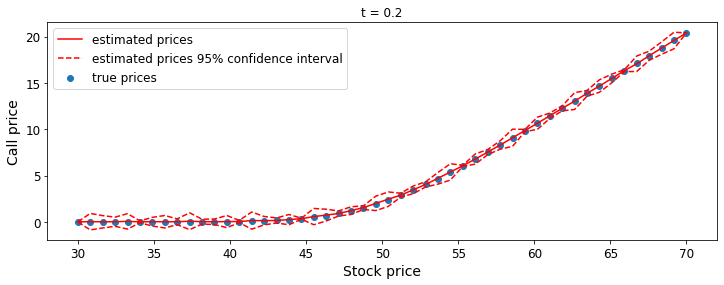
\includegraphics[width = 0.9 \linewidth]{call_price_BS_t=0.2.png}
    \caption{Estimated call prices of the trained GP model with a Matérn 5/2 kernel.}
    \label{fig:call_price_BS_t=0.2}
\end{figure}
\noindent Given the aforementioned, trained GaussianProcessRegressionModel, Delta can be found easily by computing the gradient of the posterior mean w.r.t. the underlying stock price: $\frac{\partial m^\star}{\partial S}(\mathbf{x^\star})$. The covariance of Delta can be found by the second derivative of the posterior covariance: $\frac{\partial^2 \kappa^\star}{\partial S \partial S'}(\mathbf{x^\star}, \mathbf{x'^\star})$. The analytical formulae for the Greek's mean $g_{*,j}(\mathbf{x}_*)$ and covariance $K_g(\mathbf{x}_*,\mathbf{x}'_*)$ can also be computed (depending on the chosen prior kernel function), and are given in the paper by Ludkovski and Saporito. It should be noted, however, that at the time of writing this thesis there were several small errors in those analytical formulae, notably some sign and factor errors.\\
Figure \ref{fig:delta_anal_BS_t=0.2} gives the resulting Delta estimates using the differentiated Gaussian process model. Obviously the estimated Deltas are very imprecise, and the associated confidence intervals are much too large to be reasonable. The next subsection explains why this initial implementation failed, and how it can be improved to yield more sensible results.

\begin{figure}[H]
    \centering
    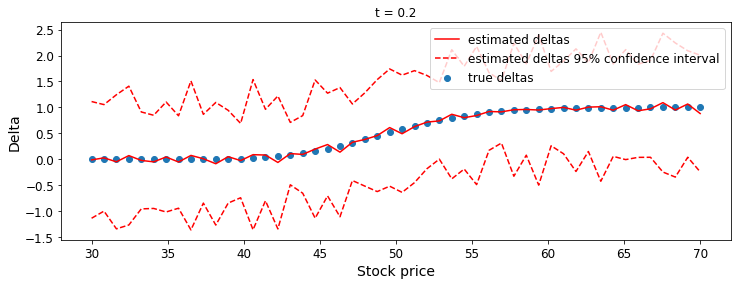
\includegraphics[width = 0.9 \linewidth]{delta_anal_BS_t=0.2.png}
    \caption{Estimated deltas using analytical formulae to derive the trained Matérn kernel.}
    \label{fig:delta_anal_BS_t=0.2}
\end{figure}

\subsubsection{Understanding the values for the Delta estimates and confidence intervals}
It might be surprising that, despite having followed the theory to the letter, our initial attempt at estimating Greeks failed so resoundingly. Naturally, the theory is still sound, and the problems come rather from the implementation. In fact, the problems are twofold.\\
The first issue lies in the \textbf{length scale parameters}. Indeed, the value of $K_g(\mathbf{x}*,\mathbf{x}'*)$ scales approximately as $1/l_{len,k}^2$ (see analytical formulas in the paper \cite{Ludkovski2020}). Thus, when the gradient descent method leads to `optimal' values of the length scale parameters that are small, the resulting confidence bounds will be inflated. Since we know more or less the scale of the two inputs, we can set boundaries on the possible values of these length scales: $l_{len,t} \in [0.1,2.0]$ and $l_{len,S} \in [10.0,50.0]$. This will ensure that the trained hyperparameters stay reasonably large, and thus that the confidence bounds stay reasonably small.\\
The second issue lies in the \textbf{sensitivity to the training data}. We recall from section \ref{sec:generating_data} that the training data we generated was shaped as a grid of equally-spaced input parameters. This is not a good idea since the prior kernels contain $(\mathbf{x}_k-\mathbf{x'}_k)/l_{len,k}$ terms, and so using equally-spaced data means that the number of possible distances $\mathbf{x}_k-\mathbf{x'}_k$ that the model can be trained on is very small. This then means that the regression algorithm can't properly train the length scale parameters. A better implementation is to use Halton sequences to generate the input parameters. These sequences are quasi-random and so allow us to avoid the problem above.\\
Figure \ref{fig:comparing_training_data} shows a side-by-side comparison of the results yielded using the previous, flawed implementation, and the new implementation, augmented by prior assumptions on the length scale parameters and by the use of Halton training data. Clearly, the estimates are now much more reasonable. The figure also shows the estimates yielded when using Monte Carlo generated prices, rather than true Black-Scholes prices. The difference between the two pricing models is that Monte Carlo prices are inherently noisy, whereas the Black-Scholes prices are noiseless. The result is that, in the new implementation, the estimates are worse; this is expected since the observation noise parameter $\sigma_\epsilon$ will be trained to be larger than in the noiseless case. However, it is perhaps less expected that, in the old implementation, the Monte Carlo data yields better results than the exact Black-Scholes data. A possible explanation for this is that adding noise to the data smooths out the estimate. Indeed, the model should learn a higher noise parameter $\sigma_\epsilon$ and will thus allow more leeway in its prediction. Since the prediction is no longer required to pass exactly through the observation points, but only near them, the resulting curve is a lot smoother. In that regard, noisy data can sometimes yield better results than noiseless data.\\
\begin{figure} [H]
     \centering
     \begin{subfigure}[b]{0.49\textwidth}
         \centering
         \makebox[0pt]{
         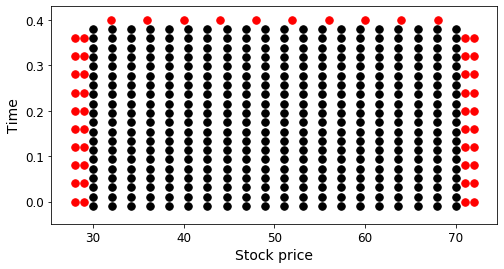
\includegraphics[width=1\textwidth]{linspace_training_points.png}}
    \caption{Linspace seq data set}
    \label{fig:linspace_training_points}
     \end{subfigure}
     \hfill
     \begin{subfigure}[b]{0.49\textwidth}
         \centering
         \makebox[0pt]{
         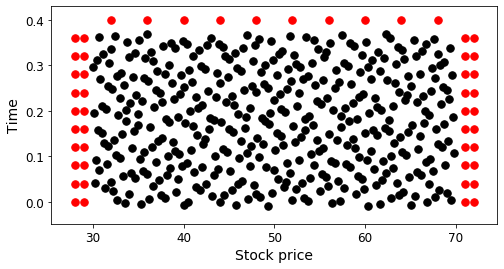
\includegraphics[width=1\textwidth]{halton_training_points.png}}
    \caption{Halton seq data set}
    \label{fig:halton_training_points}
     \end{subfigure}
     \hfill
     
     \begin{subfigure}[b]{0.49\textwidth}
         \centering
         \makebox[0pt]{
         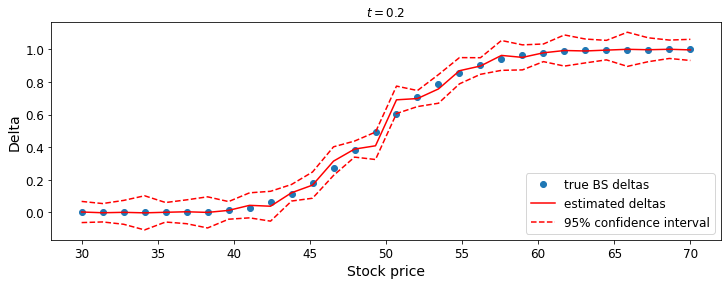
\includegraphics[width=1\textwidth]{linspace_true_prices_BS_t=0.2.png}}
    \caption{Linspace seq, true prices}
    \label{fig:linspace_true_prices}
     \end{subfigure}
     \hfill
     \begin{subfigure}[b]{0.49\textwidth}
         \centering
         \makebox[0pt]{
         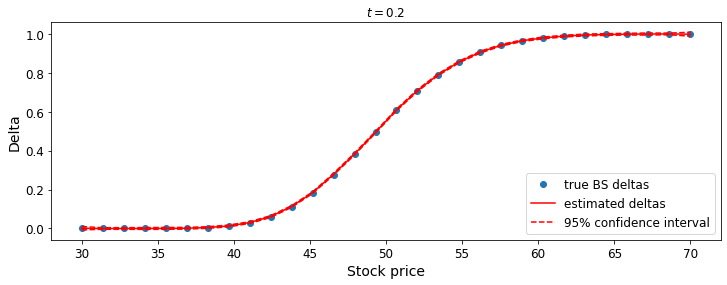
\includegraphics[width=1\textwidth]{halton_true_prices_BS_t=0.2.png}}
    \caption{Halton seq, true prices}
    \label{fig:halton_true_prices}
     \end{subfigure}
     \hfill
     
     \begin{subfigure}[b]{0.49\textwidth}
         \centering
         \makebox[0pt]{
         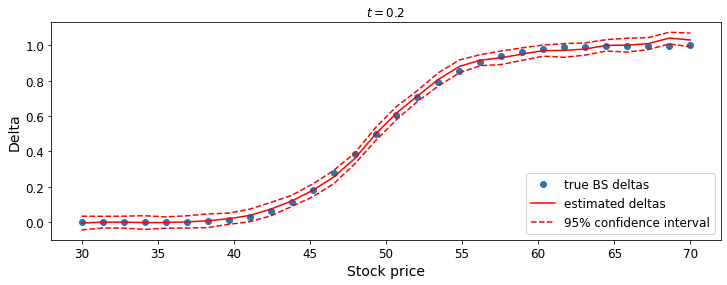
\includegraphics[width=1\textwidth]{linspace_mc_prices_BS_t=0.2.png}}
    \caption{Linspace seq, MC prices}
    \label{fig:linspace_mc_prices}
     \end{subfigure}
     \hfill
     \begin{subfigure}[b]{0.49\textwidth}
         \centering
         \makebox[0pt]{
         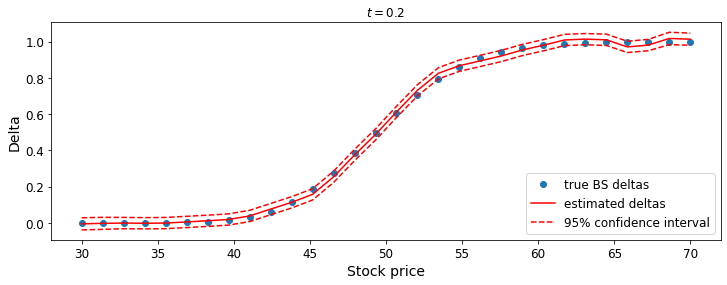
\includegraphics[width=1\textwidth]{halton_mc_prices_BS_t=0.2.png}}
    \caption{Halton seq, MC prices}
    \label{fig:halton_mc_prices}
     \end{subfigure}
    \caption{Comparing Delta values of Matern 5/2 models trained on different data. The left (resp. right) column of the figure corresponds to results yielded by an equidistant (resp. Halton) training data set. The first row presents these training data sets (the red dots are the `virtual' training points). The second row shows estimated Deltas by models trained with true Black-Scholes prices. The third row shows estimated Deltas by models trained with noisy Monte Carlo prices.}
    \label{fig:comparing_training_data}
\end{figure}
\noindent Another point of interest is that, in the case of equally-spaced data and true Black-Scholes prices, the estimates appear to be much better on the edges of the graph than in the center. Figure \ref{fig:linspace_no_virtual} shows that the added virtual points on the edge of the input grid cause the at-the-money prices to be inaccurately computed.
\begin{figure} [H]
    \centering
    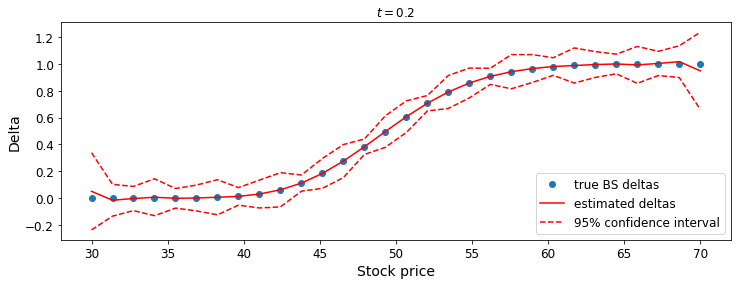
\includegraphics[width=0.75\textwidth]{linspace_true_prices_no_virtual_BS_t=0.2.png}
    \caption{Delta values for a Matern 5/2 kernel and linspace training data without virtual points and with true Black-Scholes call prices. Without the virtual points, the center of the graph looks much better.}
    \label{fig:linspace_no_virtual}
\end{figure}
\noindent Finally, figure \ref{fig:comparing_to_paper} compares the results presented in the paper by Ludkovski and Saporito to those yielded by our Python implementation. We can see that we have effectively reproduced their model in our new environment. The figure presents reasonably good estimates but, as we have shown previously, the estimates could be much improved by using true B-S prices, rather than Monte Carlo prices.\\
\begin{figure} [H]
     \centering
     \begin{subfigure}[b]{0.49\textwidth}
         \centering
         \makebox[0pt]{
         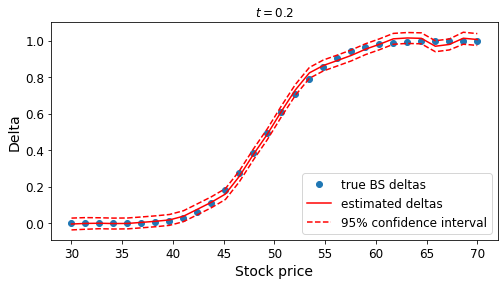
\includegraphics[width=1\textwidth]{krighedge_delta_comp.png}}
     \end{subfigure}
     \hfill
     \begin{subfigure}[b]{0.49\textwidth}
         \centering
         \makebox[0pt]{
         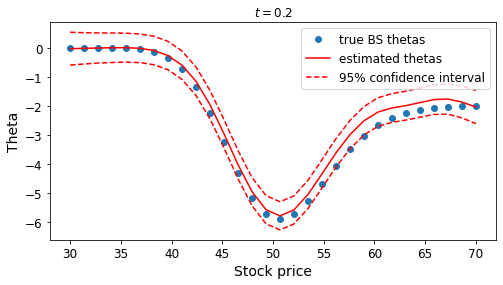
\includegraphics[width=1\textwidth]{krighedge_theta_comp.png}}
     \end{subfigure}
     \hfill
     
     \begin{subfigure}[c]{0.49\textwidth}
         \centering
         \makebox[0pt]{
         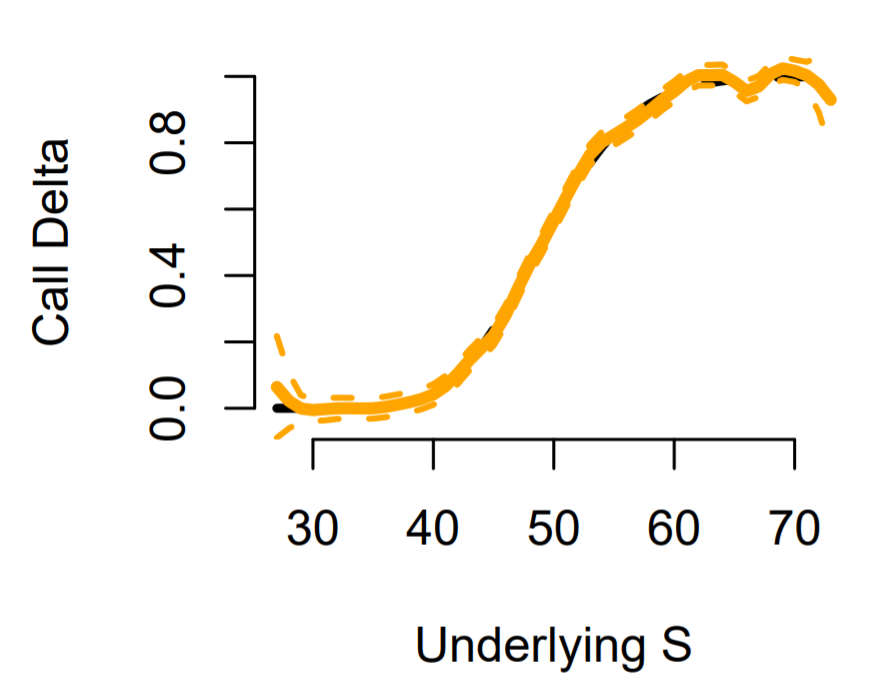
\includegraphics[width=1\textwidth]{paper_delta.png}}
     \end{subfigure}
     \hfill
     \begin{subfigure}[c]{0.49\textwidth}
         \centering
         \makebox[0pt]{
         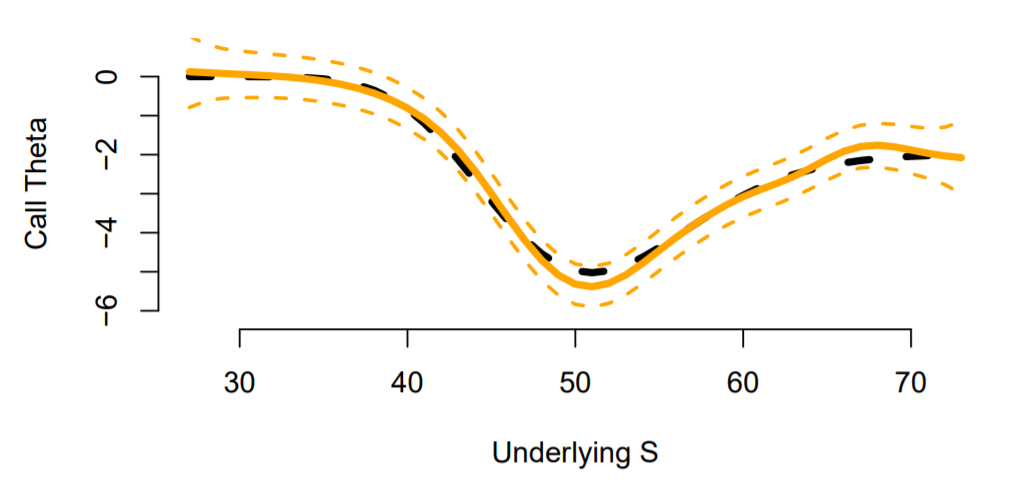
\includegraphics[width=1\textwidth]{paper_theta.png}}
     \end{subfigure}
    \caption{Comparison between the results obtained using our Python implementation (top) and the results presented in the paper \cite{Ludkovski2020} (bottom). Here the training input data is generated with a Halton sequence and the corresponding outputs are Black-Scholes Monte Carlo prices.}
    \label{fig:comparing_to_paper}
\end{figure}

\subsection{Augmenting the model with \texttt{TensorFlow}'s automatic differentiation feature}
Having successfully reproduced Ludkovski and Saporito's model, we can now add a final personal touch to our implementation that justifies our use of Python rather than R. The idea is to make use of the GradientTape feature in \texttt{Tensorflow}, which can compute gradients automatically. This would offer an alternative to computing the derivatives $\frac{\partial m^\star}{\partial S}(\mathbf{x^\star})$ and $\frac{\partial^2 \kappa^\star}{\partial S \partial S'}(\mathbf{x^\star}, \mathbf{x'^\star})$ analytically, which could be useful if, in the future, we wish to use a more complicated kernel. It also allows us to verify our analytical expressions. \\
The computation of the first derivative of the posterior mean function is easy enough. However, the computation of the second derivative of the posterior covariance is not so simple. Indeed, the Matérn 5/2 kernel contains an absolute value term $|\mathbf{x} - \mathbf{x'}|$, and for the confidence intervals we're only interested in the case where $\mathbf{x} = \mathbf{x'}$. We're therefore asking \texttt{Tensorflow} to derive the absolute value function at 0. Since this is not defined, \texttt{Tensorflow} simply returns 0. We would rather it returned either +1 or -1 (both yield the correct final expression). This is made clearer by considering the expressions of the Matérn 5/2 kernel, its first derivative, and its second derivative, which are of the form: 
\begin{align*}
    \kappa_{M52}(\mathbf{x},\mathbf{x'}) & \propto \left (1+\frac{\sqrt{5}}{l_S}|S-S'|+\frac{5}{3l_S^2}(S-S')^2 \right) e^{-\frac{\sqrt{5}}{l_k}|S-S'|}\\
    \frac{\partial \kappa_{M52}}{\partial S}(\mathbf{x},\mathbf{x'}) & \propto \left (-\frac{5}{3 l_S^2}(S-S')-\frac{5^{\frac{3}{2}}}{3 l_S^3}(S-S')|S - S'| \right) e^{-\frac{\sqrt{5}}{l_S}|S-S'|}\\
    \frac{\partial^2 \kappa_{M52}}{\partial S \partial S'}(\mathbf{x},\mathbf{x'}) & \propto \left (\frac{5}{3 l_S^2} + \frac{5^{\frac{3}{2}}}{3 l_S^3}|S - S'| - \frac{5^2}{3 l_S^4}(S-S')^2 \right) e^{-\frac{\sqrt{5}}{l_S}|S-S'|}
\end{align*}
The second derivative has a constant term since the various absolute value terms cancel out. However, since \texttt{Tensorflow} sets the derivatives of the absolute value function to 0, it will not yield this constant term. One solution to this problem would be to redefine the \texttt{Tensorflow} gradient for the absolute value function. This is actually not so quick since you need to redefine the gradient not only  w.r.t. the inputs, but also with respect to any other variable you will need the gradient for (i.e. also the hyperparameters). A less elegant, but much faster, solution is simply to define $\mathbf{x} = \mathbf{x'} + \epsilon$, where $\epsilon$ is just an arbitrarily small value. Thus we're no longer computing the gradient of the absolute value at 0, but rather at $\epsilon$.\\
Using this trick we can now use the GradientTape feature to quickly compute gradients for any and all kernels, or product or combination of kernels.

\newpage
\section{Using functional Gaussian processes to price any European option}
The first part of this thesis established the foundations of Gaussian process regression, and applied them to a simple test case. This second part now seeks to build on those foundations and apply them in a more complex scenario: the pricing of any European option. Since a European option is characterised by its payoff function, the objective is thus to create a model that can associate any input payoff function to an output price. A simple model using the finite element method is presented first, and then the concepts of that method are applied in a Gaussian process setting. The goal here is to see how well the ideas presented in the first part can be applied to a novel problem, and what the limitations of Gaussian processes might be in such a new context. Additionally, this second part of the thesis seeks to take into account the No Arbitrage conditions, and examines whether they can be used to improve the call price surface estimate yielded by the model.

\subsection{Finite element method}
Before seeing how we might implement a Gaussian process model that can price any European option, let us first establish a reference point so we can properly evaluate the performance of the GP model later. We choose the finite element method (FEM) as this reference point.
\subsubsection{Theory}
Here is reproduced in short the finite element method as described in the work ``Introduction to finite element methods" by Hans Peter Langtangen \cite{fem_paper}.\\
Suppose there is a function $f(x)$, $x \in \Omega$ which we wish to approximate. We have a set of basis functions $\phi_i(x)$ which we can linearly combine to obtain $u(x) = \sum_i \gamma_i \phi_i(x)$. Thus we wish to find the coefficients $\gamma_i$ such that $u$ is the best approximation of $f$. This is equivalent to minimising the error $E = \langle e,e\rangle$, where $e = f - u$. In the case of vectors $\mathbf{f}$ and $\mathbf{u}$, $\langle\cdot,\cdot\rangle$ is the scalar product; in the case of functions it is an integral.\\
We have:
\begin{equation}
\begin{split}
    E &= \langle e,e\rangle = \langle f-u, f-u\rangle \\
    &= \langle f,f\rangle - 2\sum_i \gamma_i \langle f,\phi_i\rangle + \sum_i\sum_j \gamma_i \gamma_j \langle\phi_i,\phi_j\rangle
\end{split}
\end{equation}
We want to minimise $E$ with respect to the parameters $\gamma_k$:
\begin{equation}
    \frac{\partial E}{\partial \gamma_k} = 0
\end{equation}
The first element is obviously 0. The second is given by:
\begin{equation}
    \frac{\partial}{\partial \gamma_k} \sum_i \gamma_i \langle f,\phi_i\rangle = \langle f,\phi_k\rangle
\end{equation}
The last element is given by:
\begin{equation}
    \frac{\partial}{\partial \gamma_k}\sum_i\sum_j \gamma_i \gamma_j \langle\phi_i,\phi_j\rangle = 2 \sum_i \gamma_i \langle\phi_i,\phi_k\rangle
\end{equation}
We write $A_{i,j} = \langle\phi_i,\phi_j\rangle = \int_{\Omega} \phi_i(x) \phi_j(x) \,dx$ and $b_i = \langle\phi_i,f\rangle = \int_{\Omega} \phi_i(x) f(x) \,dx$, and obtain:
\begin{align}
    \frac{\partial E}{\partial \gamma_k} &= 0 \\
    \iff \sum_j \gamma_j A_{i,j} &= b_i \\
    \iff A \boldsymbol{\gamma} &= \mathbf{b} \\
    \iff \boldsymbol{\gamma} &= A^{-1} \mathbf{b}
\end{align}

\subsubsection{Approximating European options with a finite set of call option data}
\paragraph{Constructing the Butterfly options}
In order to use the finite element method we must first construct a set of basis functions $\phi_i(x)$. In order for the method to work well and efficiently it is preferable to have these functions obey some basic properties. First, for a given set of points ${x_i}_{i=1}^N$:
\begin{equation}
    \phi_i(x_j) = \delta_{i,j}
\end{equation}
Second, it is preferable if $\phi_i$ is 0 when $x$ is not close to $x_i$.\\
An ideal candidate for the basis functions is the hat function defined at equally spaced $x_i = ih$, by:
\begin{equation}
    \phi_i(x) = \left\{
\begin{array}{ll}
      0 \quad x< x_{i-1} \\
      (x-x_{i-1})/h \quad x_{i-1} < x < x_i \\
      1 - (x-x_i)/h \quad x_i < x < x_{i+1} \\
      0 \quad x > x_{i+1}
\end{array} 
\right. 
\end{equation}
These hat functions are shown in figure \ref{fig:fem_hat_fcts}.
\begin{figure} [H]
    \centering
    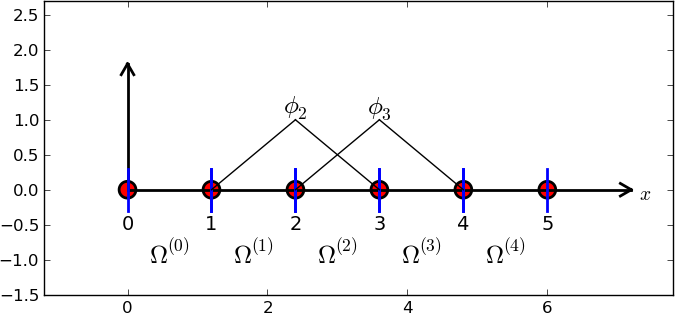
\includegraphics[width=0.9\textwidth]{fem_hat_fcts.png}
    \caption{Illustration of basis hat functions \cite{fem_paper}}
    \label{fig:fem_hat_fcts}
\end{figure}
\noindent Given a finite set of call options we therefore wish to build these hat functions. Fortunately, these functions already exist in the financial world and are called Butterfly options. A Butterfly option at strike K is defined as 
\begin{equation}
    B(K) = C(K-a) -2C(K) + C(K+a)
\end{equation}
where $a$ is just a chosen distance. Thus, with three call options we can construct our basis hat function.
\begin{figure} [H]
    \centering
    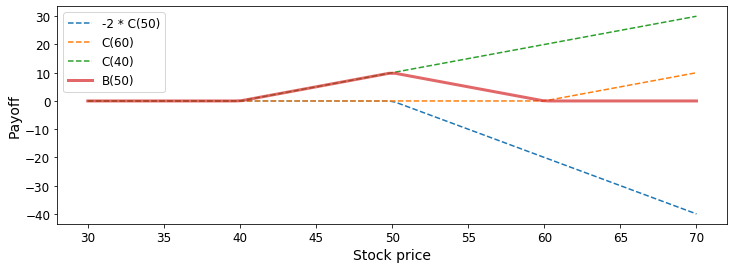
\includegraphics[width=0.9\textwidth]{butterfly_illustration.png}
    \caption{Illustration of Butterfly option construction.}
    \label{fig:butterfly}
\end{figure}

\paragraph{Approximating a new European option}
Our ultimate goal is to approximate the price $P$ of a new European option of given payoff $f(x)$. To do this, we first approximate the payoff $f(x)$ using the finite element method and our Butterfly basis:
\begin{equation}
    f(x) \approx \sum_i \gamma_i B_i(x)
\end{equation}
Then, we have:
\begin{equation}
\begin{split}
    P = \displaystyle \mathop{\mathbb{E}}_{x\in \Omega}(f(x)) &\approx \displaystyle \mathop{\mathbb{E}}_{x\in \Omega}(\sum_i \gamma_i B_i(x))\\
    &= \sum_i \gamma_i \displaystyle \mathop{\mathbb{E}}_{x\in \Omega}(B_i(x))
\end{split}
\end{equation}
Since the $B_i$ are constructed from call options for which we know the price, we can also find the price of the basis functions.

\subsubsection{Implementing the FEM}
\paragraph{Using the least squares method}
For now, let us assume that the call data we are given to generate our hat functions is regularly spaced. This allows us to compute the $A$ matrix by hand relatively quickly, for any matrix size. Indeed, if $x_i = ih$ and $\phi_i(x_i) = 1$, then 
\begin{equation}
    A = h/6 \begin{bmatrix} 
    4 & 1 & 0 & 0 & \dots & 0 \\
    1 & 4 & 1 & 0 & \dots & 0\\
    0 & 1 & 4 & 1 & \dots & 0\\
    \vdots & & & \ddots & &  \\
    0 & \dots & 0 & 0 & 1 & 4 
    \end{bmatrix}
\end{equation}
Given $N$ call prices, or data points, we can construct $N-2$ Butterfly options. These Butterflies are also divided by $h$ in order to produce perfect hat functions that peak at a value of $1$ rather than $h$. Using the \texttt{scipy.integrate.quad} function in Python, we compute $b_i = \langle\phi_i,f\rangle = \int_{\Omega} \phi_i(x) f(x) \,dx$ for each hat function. Figure \ref{fig:fem_varying_N} shows how well the payoff of a call function at strike $K=52$ is approximated by the finite element method, for varying number $N$ of data points in the range $K \in [30, 70]$. The range of the test points is chosen to be smaller ($[35, 65]$) since the first and last data point of the basis set are discarded to build the basis functions. It is interesting that beyond a certain point, the approximation becomes worse for large $N$. This might be due to the integration function of the \texttt{scipy} package. Indeed, as more data points are added, the hat functions become more and more narrow with respect to the domain (which is fixed). Thus they begin to resemble Dirac delta functions which are difficult to integrate.

\begin{figure} [H]
    \centering
    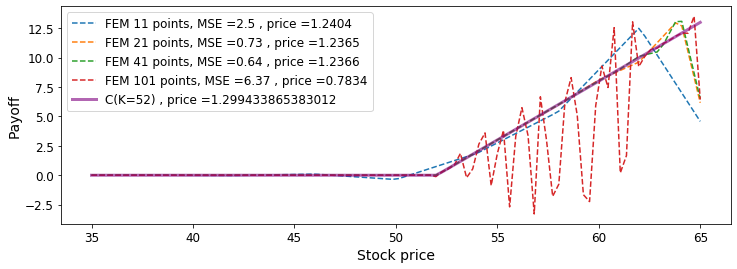
\includegraphics[width=0.9\textwidth]{fem_approx_varying_N_hat.png}
    \caption{Approximation of call function payoff using the FEM with varying number of data points. The mean squared error of each approximation is given, as well as the predicted price.}
    \label{fig:fem_varying_N}
\end{figure}

\paragraph{Using the interpolation (or collocation) method}
Since integrating the hat functions numerically is problematic, an alternative solution is to use the interpolation method \cite{fem_paper}. Here, we require that our approximation $u(x) = \sum_i \gamma_i \phi_i(x)$ passes through some select points, namely: $u(x_i) = f(x_i)$. We obtain the same linear system as before $A\boldsymbol{\gamma} = \mathbf{b}$, but now the coefficients have changed: $A_{i,j} = \phi_j(x_i)$ and $b_i = f(x_i)$. With this method we no longer need to compute integrals. In addition, we can select the points $x_i$ to coincide with the peaks of our hat functions. In this case, the matrix $A$ becomes the identity matrix and we have $\gamma_i = f(x_i)$. Figure \ref{fig:fem_interpolation} illustrates the approximation produced using this method, for the same call function as in the previous method. Clearly, this method works much better, or at least it does in a numerical setting where computing integrals can be difficult.
\begin{figure} [H]
    \centering
    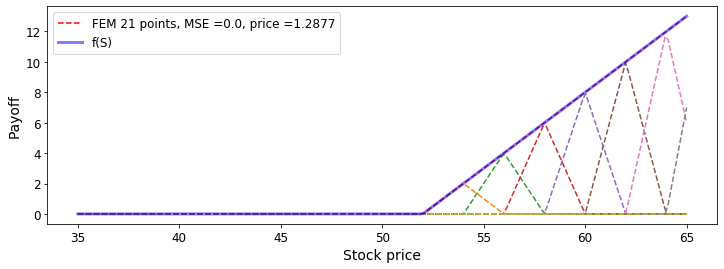
\includegraphics[width=0.9\textwidth]{fem_interpolation_C52.png}
    \caption{Approximation of call function payoff with strike $K=52$ using the interpolation method. The mean squared error is 0.0 implying a perfect fit on the $[35,65]$ range; the approximated price is slightly lower than the theoretical price since the basis data points stop after $K=70$.}
    \label{fig:fem_interpolation}
\end{figure}

\subsection{Functional Gaussian processes}
Having presented a simple first attempt using the finite element method, we now try to solve the same pricing problem using Gaussian process regression. The idea is to approximate a functional that takes as input a payoff function, and gives as output the price associated to that payoff function. Whereas in section \ref{sec:ludkovski} the Gaussian processes took scalars $(t, S)$ as inputs (or vectors of scalars), a functional Gaussian process takes functions as inputs.

\subsubsection{Theory}
This part is mainly a summary of the concepts described in the paper by Nguyen and Peraire \cite{fgp_paper}.\\
We wish to approximate a functional $g$ which we represent as a Functional Gaussian Process (FGP) of zero mean and covariance operator $k$: $g(v) \sim \mathcal{FGP}(0, k(v,v')), \quad v, v' \in V$. Here $V$ is a space of input functions to our functional. The covariance operator $k$ needs to be symmetric positive definite; one such operator is the integral: $k(v,v') = \theta \int_\Omega v(x) v'(x) dx$, where $\Omega$ is the domain over which the function space $V$ is defined, and $\theta$ is a hyperparameter.\\
Similarly to the classical Gaussian Process case, we can define a regression procedure given training data $\boldsymbol{\Phi} = [\phi_1, \phi_2, ..., \phi_M]$ with corresponding observed outputs $\mathbf{y}$, and test data $\boldsymbol{\Phi^*} = [\phi^*_1, \phi^*_2, ..., \phi^*_{M^*}]$.\\
We define:
\begin{equation}
\begin{aligned}
  g_i &= g(\phi_i)\\
  g^*_i &= g(\phi_i^*)\\
  K_{ij}(\boldsymbol{\Phi}, \boldsymbol{\Phi}) &= k(\phi_i,\phi_j)\\
  K_{ij}(\boldsymbol{\Phi^*}, \boldsymbol{\Phi}) &= k(\phi^*_i,\phi_j)\\
  K_{ij}(\boldsymbol{\Phi}, \boldsymbol{\Phi^*}) &= k(\phi_i,\phi^*_j)\\
  K_{ij}(\boldsymbol{\Phi^*}, \boldsymbol{\Phi^*}) &= k(\phi^*_i,\phi^*_j)\\
\end{aligned}
\end{equation}
Then we can write the posterior distribution $\mathbf{g^*}|\mathbf{y},\boldsymbol{\Phi},\boldsymbol{\Phi^*} \sim \mathcal{N}(\mathbf{\Bar{g}^*}, \text{cov}(\mathbf{g^*}))$, where:
\begin{equation}
\label{fgp_posterior_mean}
    \mathbf{\Bar{g}^*} = \mathbf{K}(\boldsymbol{\Phi^*}, \boldsymbol{\Phi})(\mathbf{K}(\boldsymbol{\Phi}, \boldsymbol{\Phi}) + \sigma^2 \mathbf{I})^{-1}\mathbf{y}
\end{equation}
\begin{equation}
\label{fgp_posterior_cov}
    \text{cov}(\mathbf{g^*}) = \mathbf{K}(\boldsymbol{\Phi^*}, \boldsymbol{\Phi^*}) - \mathbf{K}(\boldsymbol{\Phi^*}, \boldsymbol{\Phi})(\mathbf{K}(\boldsymbol{\Phi}, \boldsymbol{\Phi}) + \sigma^2 \mathbf{I})^{-1}\mathbf{K}(\boldsymbol{\Phi}, \boldsymbol{\Phi^*})
\end{equation}
The functional regression method is much the same as the classical one we've already seen: having defined a prior distribution we use the training data to train the hyperparameters by maximising the log marginal likelihood; we then compute the posterior distribution using formulas \ref{fgp_posterior_mean} and \ref{fgp_posterior_cov}.

\subsubsection{Implementation}
Given the similarities between the functional method and the classical method, the implementation is relatively straightforward, although there is a complication. The first thing to do is to define a covariance operator; we choose the aforementioned integral. To implement an integral in python we simply use a rectangles method:
\begin{equation}
    \int_\Omega y(x) dx = \sum_{i=0}^{N-1} \frac{y(x_i) + y(x_{i+1})}{2} dx
\end{equation}
where we've partitioned the continuous space $\Omega$ into a discrete space $\{x_i\}_{i=0}^N$.\\
The next step is to generate our training data. We choose the same Butterfly functions we used for the finite element method; these are our input functions. Their Black-Scholes prices will be our observation outputs $\mathbf{y}$. Here, however, arises the complication. We wish to use the existing \texttt{TensorFlow} package since it does the hyperparameter optimisation and the posterior distribution computation automatically. The problem is that functions cannot be converted to tensors. Therefore, instead of inputting the functions $\phi_i$ into the FGP, we input the array $\{\phi_i(x_j)\}$ where the $x_j$ correspond to the discretisation of the space $\Omega$. Given the definition of our integral, and therefore our covariance function, these function values are all that we need anyway. Likewise we also need to discretise our test data.

\subsubsection{Results}
It should be noted that the point of view presented in the graphs in this section, and every section from here till the end of the thesis, has changed with respect to the point of view of section \ref{sec:ludkovski}. Indeed, in their paper \cite{Ludkovski2020} Ludkovski and Saporito elect to use the spot price $S$ and the time $t$ as inputs to their model, and plot their graphs according to these variables. This makes sense in the context of the paper since they are concerned with Greeks, which are defined as derivatives of the option price with respect to these two variables. However, in a more general sense it is common to consider price surfaces w.r.t. strike price $K$ and time-to-maturity $T$, rather than $(t, S)$. As such, we will now take the more common point of view and plot all our graphs w.r.t. $(T, K)$. In fact, currently the model we have defined only takes as input a payoff function (this corresponds to the $K$ dimension), but does not yet take as input the $T$ dimension. This feature will be added later; till then we consider the time-to-maturity fixed at $T = 0.2$.
\begin{figure} [H]
    \centering
    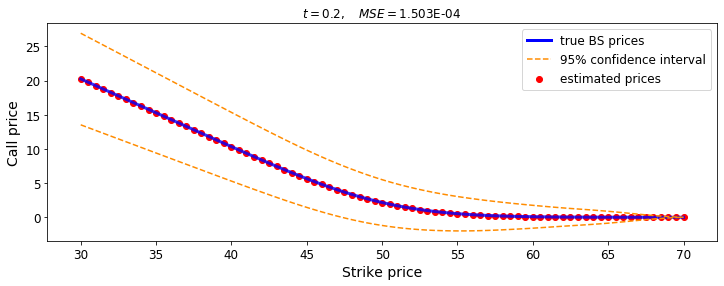
\includegraphics[width=0.9\textwidth]{fgp_call_price_approx.png}
    \caption{Functional Gaussian process approximation of call prices for varying strikes. The Mean Squared Error between the two curves is also given.}
    \label{fig:fgp_call_price_approx}
\end{figure}

\paragraph{The impact of the size of the training space on call price estimates}
The first point of interest is to see how well this new functional Gaussian process model matches up against the previous finite element method. Figure \ref{fig:fgp_call_price_approx} thus shows the FGP approximation of call prices for different strikes, when the model was trained on 9 Butterfly options. The approximation is perfect, although the confidence intervals seem abnormally large. To compare, using the same 9 basis functions and the same test range $[30, 70]$, the finite element method yields a call price curve estimate with a mean squared error of $2.176 \times 10^{-3}$, about one order of magnitude worse than the Gaussian process estimate.

\noindent A possible explanation for the large confidence bounds in figure \ref{fig:fgp_call_price_approx} lies in the size of the training space. Until now the training set of Butterfly options was built on the $K \in [30, 70]$ range. The test set of call options was also built on this range. In fact, because you cannot build a Butterfly option centered on the first and last strike in the set, the training set range is even smaller than the test set range. This means that in figure \ref{fig:fgp_call_price_approx}, the model is actually extrapolating on a few values, which could explain the abnormally large confidence bounds. In figure \ref{fig:fgp_call_price_approx_linspace} the training set range has been increased to $[25, 75]$ (keeping the same number of training functions), while the test set is still fixed at $[30, 70]$. The confidence bounds are here much more reasonable. It therefore appears that, similarly to the FEM, the functional Gaussian process works well when interpolating but breaks down during extrapolation.
\begin{figure} [H]
    \centering
    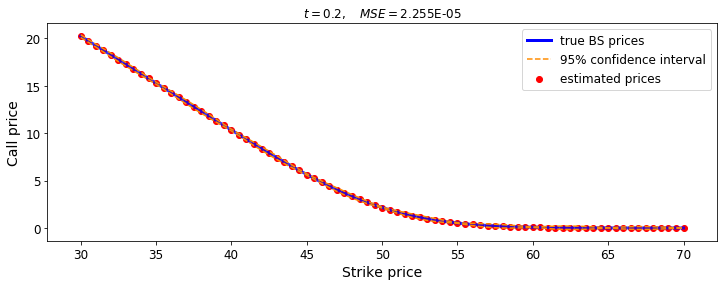
\includegraphics[width=0.9\textwidth]{fgp_call_price_approx_linspace_.png}
    \caption{FGP approximation of call prices for varying strikes where the model was trained on a larger range than the test set. The Mean Squared Error between the two curves is also given.}
    \label{fig:fgp_call_price_approx_linspace}
\end{figure}

\paragraph{Pricing various payoff functions}
Having tested the FGP model against call prices, it would be interesting to see how well it can price a larger variety of payoff functions. Indeed, there are already countless models that can price calls, but a model that can price any European option is not so common. Table \ref{table:various_payoffs} collects the prices approximated by the FGP model, trained on 9 Butterfly functions, for various inputted payoff functions. The FGP estimate is compared to a finite element method estimate using only 9 basis functions. The `true' price corresponds to the estimate given by the finite element method, using $ 10000 $ basis hat functions.
\begin{table}[H]
\begin{center}
\resizebox{1\linewidth}{!}{
\begin{tabular}{ |c||c|c|c|c|  }
 \hline
 Payoff function & FGP estimated price & FGP estimated std dev. & FEM estimated price & True price \\
 \hline
  $f(x) = \exp \left(-\frac{(x-50)^2}{2 * 10^2} \right)$ & 0.88851 & 0.0033543 & 0.87917 & 0.88868\\
 \hline
  $f(x) = x^2$ & 2543.8 & 9.0252 & 2541.5 & 2542.8\\
  \hline
  $f(x) = \text{cos}(x)+1$ & 1.0202 & 0.33957 & 1.0044 & 0.99172\\
  \hline
  $f(x) = 
    \begin{cases}
      0 \quad \text{if} \ x < 50\\
      1 \quad \text{if} \ x \geq 50
    \end{cases}$ & 0.51057 & 0.067152 & 0.66241 & 0.50854\\
  \hline
\end{tabular}}
\end{center}
\caption{FGP price approximation for various payoff inputs compared to a FEM price approximation and a `true' price.}
\label{table:various_payoffs}
\end{table}
\noindent The FGP model performs quite well, even when its estimated standard deviation is high like with the cosine function. The FGP model performs similarly to (or sometimes slightly better than) the FEM for the first three test payoff functions, but it performs considerably better for the last example. This suggests that the FGP model is more versatile than the FEM, and that it handles discontinuous data much better.

\paragraph{Choosing a better set of training functions}
Until now we have been mirroring the basis functions of the FEM by using Butterfly options as training data for our model. This was interesting in so far as it allowed us to compare the FEM and the FGP model, but it is not the best choice of training functions for our model. Indeed, as we have seen, using Butterfly functions as training data can lead to issues on the extremities of the strike price domain, and gives nonsensical confidence bounds when extrapolating. In addition, building the Butterfly functions forces us to discard two call option points (the first and the last). Given that call option data is often already limited, throwing away two training points seems wasteful. Lastly, in the rest of this section we will focus mainly on call options, and trying to apply No Arbitrage conditions on the estimated call option prices. This all indicates that using call options as the input data to our FGP model is a much more judicious choice than Butterfly options. Thus, from now on it should be assumed that all FGP models are trained on call functions rather than Butterflies, unless specified otherwise.

\subsubsection{Deriving the No Arbitrage conditions \label{sec:na_cond_proof}}
Now that we have a functioning and tested framework for the functional Gaussian process, it is time to build upon it by introducing the notion of No Arbitrage conditions.\\
In finance, an arbitrage represents an opportunity to make a positive return with a non-zero probability, and with zero probability of making a negative return. In other words, in a world where `there is no such thing as a free lunch', an arbitrage is the possibility of a risk-free profit. Naturally, any economically-sound pricing model must not output prices that result in an arbitrage opportunity. In section \ref{sec:ludkovski}, we did not take into account arbitrage opportunities, but now we shall try to implement `No Arbitrage' conditions into our FGP model. A No Arbitrage condition is a condition that, if broken, indicates an arbitrage opportunity. As such, any sound model must fulfil these conditions; even then it is not guaranteed that the model is arbitrage-free, but at the very least some arbitrage opportunities will have been removed.\\
The paper by Niu \cite{NA_cond_all} lists the No Arbitrage conditions on the call price surface. From that list, we shall focus only on the two following conditions:
\begin{enumerate}
    \item The price of a call option is convex in strike.
    \item The price of a call option is monotone increasing in time-to-maturity.
\end{enumerate}
The proof for the first condition is given in the paper by Touzi and Tankov \cite{NA_cond_K}, but I will rewrite it here:
\begin{proof}
A function $f : X \rightarrow \mathcal{R}$ is convex if and only if $\quad \forall \lambda \in [0, 1],\ \forall x_1, x_2 \in X,$ $$ f(\lambda x_1 + (1-\lambda) x_2) \leq \lambda f(x_1) + (1-\lambda) f(x_2)$$
Notice that this is verified for the intrinsic value of a call option: 
$$\lambda |S-K_1|_{+} + (1-\lambda) |S-K_2|_{+} - |S-\lambda K_1 - (1-\lambda) K_2|_{+} \geq 0 $$
We can thus construct a portfolio by going long $\lambda$ calls with strike $K_1$ and $(1-\lambda)$ calls with strike $K_2$, and by going short one call with strike $\lambda K_1 + (1-\lambda) K_2$. By the inequality above, the value of this portfolio is never negative and so we must have 
$$C(\lambda K_1 + (1-\lambda) K_2) \leq \lambda C(K_1) + (1-\lambda) C(K_2)$$
where $C(K)$ is the price of a call option at strike $K$, otherwise there would be an arbitrage.\\
Hence the convexity of the call option price is a no arbitrage condition.
\end{proof}
~\\
The proof for the second condition is given in the paper by Merton \cite{Merton1973}, but I will write a modified version here:
\begin{proof}
It is obvious that the condition $C(T_2) > C(T_1)$, for $T_2 > T_1$, must be verified for American call options since one could always exercise the call option with longer maturity $T_2$ early at time $t \leq T_1$. It also turns out that, when considering a stock that yields no dividends, the price of an American call option is equal to the price of a European call option. Given that statement, the monotonicity condition is also verified by European call options. The proof of that statement lies in the fact that for a stock yielding no dividends, it is never optimal to exercise an American call option early.\\
Consider two portfolios A and B: the first consists of an American option of strike $K$ and maturity $T$ and $K e^{-r(T-t)}$ in cash; the second consists of only the stock $S$.\\
At a time $t < T$, the value of the first portfolio is:
$$ V_A = |S - K|_{+} + K e^{-r(T-t)} < S - K + K e^{-r(T-t)} < S = V_B $$
At time $t = T$, the value of the first portfolio is:
$$ V_A = \text{max}(S-K, 0) + K = \text{max}(S, K) \geq S = V_B$$
It follows that one should never exercise at $t < T$.
\end{proof}

\subsubsection{Implementing the No Arbitrage condition for the strike dimension}
Since our model is, at this point, only dependent on the strike price $K$, we only need to implement the first No Arbitrage condition: that the price of a call option is convex in strike.
\paragraph{Rejecting non-convex samples}
The first idea to enforce the No Arbitrage condition on our model is to simply reject the samples yielded by the model that break the condition, and keep those that satisfy it. Figure \ref{fig:fgp_concave_points} shows the mean curve of the FGP and a single sampled curve from the same FGP. It also shows the points where the sampled curve is non-convex, according to a finite differences method. The mean curve has no such points and is therefore fully convex. Nonetheless, just because the mean function was convex in this example doesn't mean it always will be. It would be much better to construct a mean from samples that have been verified as convex. The resulting mean would then also be guaranteed to be convex since a sum of convex curves is also convex. The problem is that our FGP model doesn't seem to ever output fully convex samples, as seen in figure \ref{fig:fgp_concave_points}. So, the idea of generating samples randomly until a fully convex sample is yielded would at best take a prohibitively long time, and at worst would never yield such a sample. This problem is only made worse by the fact that we would require many such samples to construct our mean. All in all, this method does not seem feasible.
\begin{figure} [H]
    \centering
    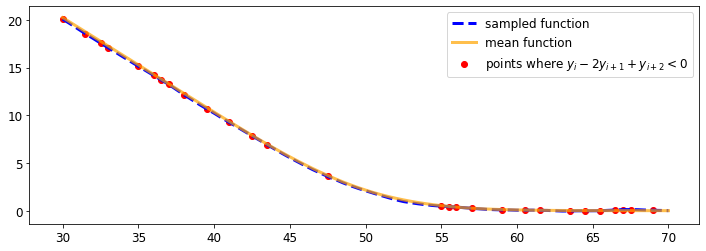
\includegraphics[width=0.9\textwidth]{na_cond_concave_points.png}
    \caption{Points where the curve sampled from the FGP is non-convex. The mean curve has no such points.}
    \label{fig:fgp_concave_points}
\end{figure}

\paragraph{Using MCMC methods}
Another idea is to use Markov Chain Monte Carlo methods to generate convex samples. The `main' MCMC method is called the `Metropolis-Hastings' algorithm. This algorithm starts with a sample (in our case a vector of $n$ call prices associated to varying strikes) and produces another sample that depends directly on the previous one. At each step it produces an entirely new sample (i.e. an entirely new vector). This is problematic for us since this new vector will presumably have the same problem as before: too many non-convex points. This method of generating samples is therefore akin to the simple rejection method described above, and would take a similarly large number of steps to produce even one completely convex sample.\\
Another MCMC method is called `Gibbs sampling'. In this method, instead of generating the whole sample/vector in one go, each step consists in changing the value of only one element at a time. In this way, instead of the whole $n$ points needing to satisfy the conditions, we only need one point to satisfy them at each step. The problem with this method is that it only really works if the initial sample is already convex, which defeats the point. Also, after a short test run it became apparent that the new samples tended to remain almost or exactly equal to the initial convex sample.\\
Thus it is not clear at this point how MCMC methods can be used to directly sample convex curves efficiently. Some papers \cite{lopezlopera} \cite{Chataigner2020BeyondSM} outline models that employed these methods, but not in the context of a functional Gaussian process as we are using here.

\paragraph{Projecting non-convex samples onto convex curves \label{sec:na_projection}}
An alternative to sampling convex samples is to simply project the non-convex samples onto the set of convex curves, in order to obtain their nearest convex approximation. The problem becomes: given a non-convex curve $f$, find the curve $f'$ that minimises $|f-f'|$ such that $f'(K-h) - 2 f'(K) + f'(K+h) \geq 0 \quad \forall K, h$. Note that the distance $|f-f'|$ is here evaluated as the Euclidean norm of $f-f'$. As a possible extension, it might be interesting to explore using a weighted norm (with larger weights for at-the-money prices, and smaller weights elsewhere).\\
Given that our `curves' are actually finite dimensional vectors, there are a finite number of conditions. This problem can be solved using the Python package \texttt{scipy.optimize}. This package uses a number of different minimisation algorithms; we choose the `Trust-region Constrained' algorithm \cite{scipy.optimise}. Figure \ref{fig:fgp_projected_sample} shows the resulting convex approximation of an initial non-convex curve. In order for the difference to be visible, the FGP model was only trained on 5 call functions (note: not Butterfly options), which leads to large confidence bounds and so very `wavy' samples. In figure \ref{fig:fgp_projected_mean}, the mean of the projected curves of 300 non-convex samples is given. Naturally, as the number of samples increases, the projected mean tends towards the initial mean of the non-convex curves; this is reassuring as it is what we would have expected.
\begin{figure} [H]
    \centering
    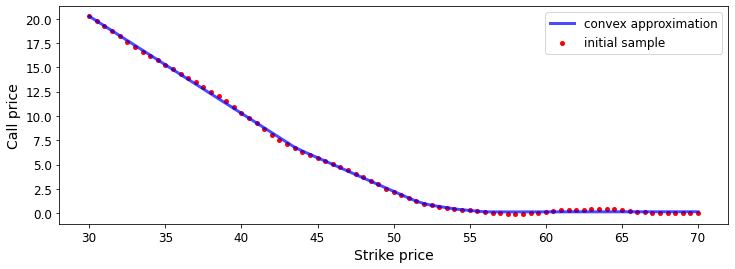
\includegraphics[width=0.9\textwidth]{fgp_projected_sample.png}
    \caption{Projection of a non-convex sample onto a convex curve.}
    \label{fig:fgp_projected_sample}
\end{figure}
\begin{figure} [H]
    \centering
    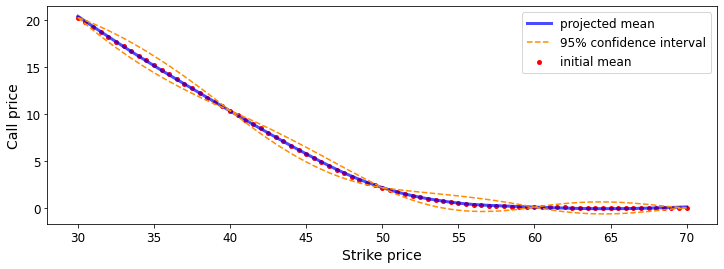
\includegraphics[width=0.9\textwidth]{fgp_projected_mean.png}
    \caption{Mean of the projections of 300 non-convex samples, and corresponding confidence bounds.}
    \label{fig:fgp_projected_mean}
\end{figure}

\subsubsection{Adding the time component}
\paragraph{Theory}
Until now we have been generating option prices for fixed time-to-maturity. It is rather straightforward to extend the existing model to allow a time component by realising that multiplying two valid kernels yields another valid kernel. Therefore we can keep the current kernel and simply multiply it by a standard Gaussian kernel that takes as input the time-to-maturity. The input to the generalised model now becomes a vector of payoff function values (as before) and a scalar representing the time component. By choosing a Gaussian kernel for the time component we only add one hyperparameter: the time length scale $l_T$. Our combined kernel thus looks like this:
\begin{equation}
    k(v, v', T, T') = \theta \int_\Omega v(x) v'(x) dx \cdot \exp \left( -(T-T')^2/(2*l_T^2) \right)
\end{equation}
Generating the training and test data is equally straightforward: we once again create a grid of $(T, K)$ values (like in section \ref{sec:generating_data}). For each point on the grid we evaluate the payoff function $f(T,K,S_i)$ at $\{S_i\}_{i=1}^n$ points, like in the previous 1D FGP; we then add the time-to-maturity as an input. Our full input vector now looks like: $[f(T,K,S_1), ..., f(T,K,S_n), T]$. The output of the model is still just a scalar corresponding to the price of the payoff function $f(T,K)$ for each point $(T, K)$ on the grid.

\paragraph{Results}
Naturally, having extended the input domain to two dimensions, we need to use more data to train the model. Previously we had been training it using approximately 10 payoff functions at a fixed time-to-maturity; now we train it on 10 payoff functions (specifically call functions) at 10 different time-to-maturities. We thus have 100 input training functions. We also use a Halton sequence to generate the $(T, K)$ grid, since this allows better training of the hyperparameters, as seen in section \ref{sec:ludkovski}.\\
\begin{figure} [H]
    \centering
    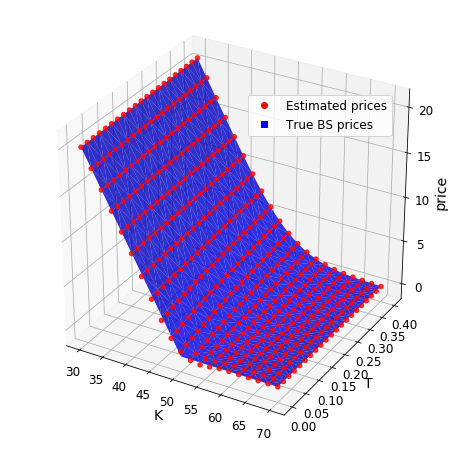
\includegraphics[width=0.6\textwidth]{fgp_2d_price_surface.png}
    \caption{Estimated call price surface yielded by the 2-dimensional FGP model.}
    \label{fig:fgp_2d_price_surface}
\end{figure}
\noindent Figure \ref{fig:fgp_2d_price_surface} shows the resulting call price surface. Unfortunately, the confidence bounds are difficult to view in 3D. Figure \ref{fig:fgp_2d_varying_T_K=39} thus shows a call price curve for fixed $K$ and varying $T$, where the strike price does not correspond to a training point, meaning the error in $K$ should be non-zero. The estimated prices are fairly close to the true prices, although they start to deviate for very small time-to-maturity. Interestingly, the confidence bounds don't seem to fluctuate much with $T$; they depend almost solely on the value of $K$. This might indicate that the estimated error is dominated by the strike dimension, and therefore that the fluctuations in the error in the time dimension are so small as to be unnoticeable. This hypothesis is confirmed by figure \ref{fig:fgp_2d_varying_T_K=38} which shows the same call price curve for varying $T$, but this time the strike is fixed at a training point value, meaning the error in $K$ should be zero. We now see the error fluctuations in the time dimension. Clearly, the error in $T$ is much smaller than the error in $K$, observed in figure \ref{fig:fgp_2d_varying_T_K=39}, except at the smaller time-to-maturity values where the errors are about equal. This indicates that it is perhaps more judicious to include more training points in the $K$ dimension than in the $T$ dimension, or else to include more training points at smaller values of $T$ rather than distributing them evenly across the input range. This redistribution of training points would help reduce the estimated error where it is largest.\\

\begin{figure} [H]
    \centering
    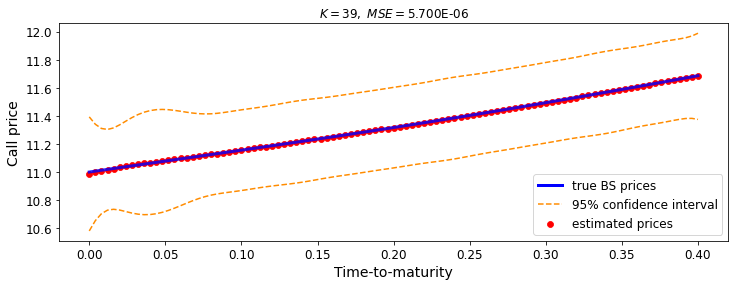
\includegraphics[width=0.9\textwidth]{fgp_2d_varying_T_K=39.png}
    \caption{Estimated call price curve yielded by the 2-dimensional FGP model for varying time-to-maturity and fixed strike. The strike price \textit{does not} correspond to a training point, meaning the error in $K$ should be non-zero.}
    \label{fig:fgp_2d_varying_T_K=39}
\end{figure}
\begin{figure} [H]
    \centering
    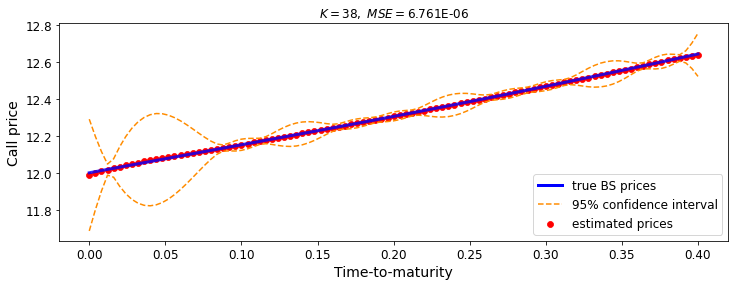
\includegraphics[width=0.9\textwidth]{fgp_2d_varying_T_K=38.png}
    \caption{Estimated call price curve yielded by the 2-dimensional FGP model for varying time-to-maturity and fixed strike. The strike price here \textit{does} correspond to a training point, meaning the error in $K$ should be zero and only the error in $T$ should remain.}
    \label{fig:fgp_2d_varying_T_K=38}
\end{figure}

\paragraph{Implementing the No Arbitrage conditions in two dimensions}
The previous method in section \ref{sec:na_projection} was to project non-convex samples onto convex curves using a \texttt{scipy} optimisation function. This method is still valid in two dimensions, albeit with certain adjustments required. Whereas before we simply had a vector of inputs $[(T,K_1), ..., (T,K_n)]$ and therefore also a vector of outputs, we now have a grid of inputs and a grid of corresponding outputs. Suppose our $(T, K)$ grid has size $(N_T \times N_K)$, then the no arbitrage conditions can be determined as follows:\\
\begin{enumerate}
    \item Convexity conditions: Iterate over every time $\{T_i\}_{i=1}^{N_T}$. For each $T_i$ iterate over the strikes $\{K_j\}_{j=1}^{N_K}$ and impose $P(T_i, K_j) - 2*P(T_i, K_{j+1}) + P(T_i, K_{j+2}) \geq 0$, where $P(T, K)$ is the price of the call option $C(T, K)$. As such, we have $N_T*(N_K-2)$ convexity conditions (we can't count the two external strikes). 
    \item Monotonicity conditions: Iterate over every $K_j$ and $T_i$ and impose $P(T_{i+1}, K_j) - P(T_i, K_j) \geq 0$. As such, we have $N_K*(N_T-1)$ monotonicity conditions (we can't count the last time-to-maturity).
\end{enumerate}
Since the optimisation function only takes in vectors and not matrices the task becomes slightly more difficult, but by flattening the matrix and using a strided iteration we can implement the above conditions.\\
Figure \ref{fig:2d_na_conditions} shows a side-by-side comparison of an estimated price surface and its corresponding No Arbitrage projection. Note that the mean squared error has halved with the projection meaning we are closer to the true prices. This is reassuring as it shows that the projection method does actually help to improve our estimations whilst also ensuring that these estimations are not economically nonsensical.

\begin{figure}[H]
\begin{minipage}[c]{.45\linewidth}
    \centering
    \makebox[0pt]{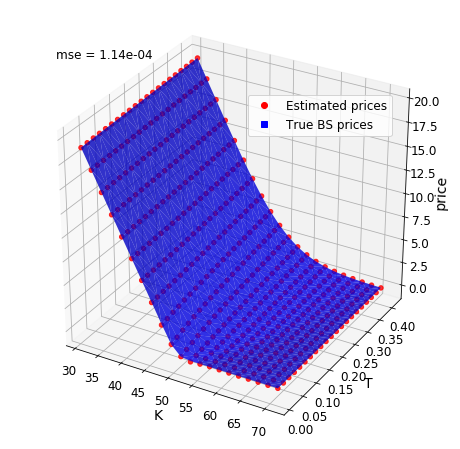
\includegraphics[width = 8.5 cm]{fgp_2d_price_surface_shifted.png}}
\end{minipage} \hfill
\begin{minipage}[c]{.45\linewidth}
    \centering
    \makebox[0pt]{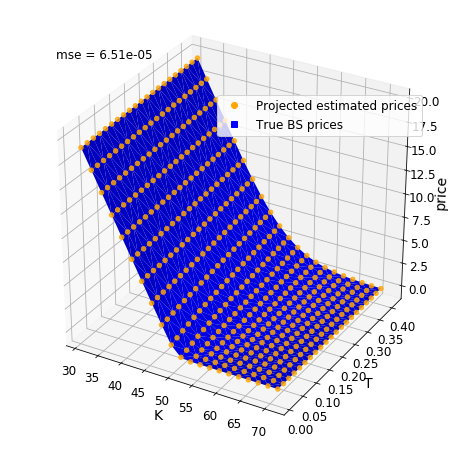
\includegraphics[width = 8.5 cm]{fgp_2d_price_surface_shifted_NA.png}}
\end{minipage}
\caption{The plot on the left shows the call price surface estimated by the FGP model, trained on a grid of 100 $(T, K)$ points. The plot on the right shows the same price surface after it has been projected onto a surface that respects the No Arbitrage conditions.}
\label{fig:2d_na_conditions}
\end{figure}

\paragraph{Using real market data}
The final test of the FGP model is to see how it fares outside of the simplistic Black-Scholes model we've been using so far. To this end, we now train and test the model using real historical option data obtained from \cite{histoptiondata}. Specifically we use prices for American calls on Amazon stock sold on 02/11/2018, at which time the price of the underlying was $\$1665.53$. The option prices we use are actually the midpoint between the quoted bids and asks. The data we obtain is shown in figure \ref{fig:real_data_amzn_grid}. Clearly, this data is a lot less regular than the previous Black-Scholes data. Note that there was actually an abundance of different strikes (over 500 different strike values compared to only 15 time-to-maturity values). However, in the interest of comparing the results using real data to the previous results using B-S data, we have restricted the training data to a $(11 \times 11)$ grid instead of the potential $(500 \times 15)$ grid.
\begin{figure} [H]
    \centering
    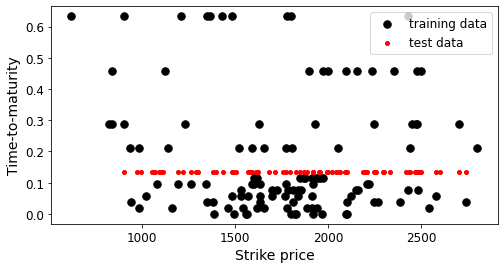
\includegraphics[width=0.7\textwidth]{real_data_amzn_grid.png}
    \caption{Training and test data set of real historical call options on Amazon stock.}
    \label{fig:real_data_amzn_grid}
\end{figure}
\begin{figure} [H]
    \centering
    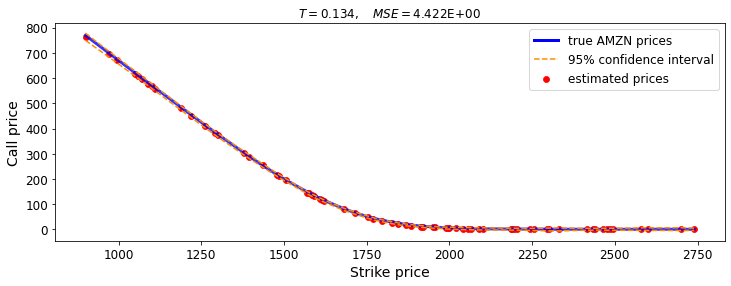
\includegraphics[width=0.9\textwidth]{real_data_amzn_call.png}
    \caption{Estimated call prices yielded by the 2-dimensional FGP model trained on real call option data.}
    \label{fig:real_data_amzn_call}
\end{figure}
\noindent Figure \ref{fig:real_data_amzn_call} shows the estimations of call prices for our test data set, using the FGP model trained on market data. At first glance the estimation looks reasonable, as do the confidence bounds. However, the mean squared error is significantly higher when using market data than it was for Black-Scholes data, even if one takes into account the relatively high underlying stock price ($S = 50$ for B-S data compared to $S = 1665$ for market data). Figure \ref{fig:real_data_amzn_put} shows a similar graph but here for put option prices. Here the estimations are noticeably worse than for calls, which makes sense since the model was trained using call options rather than put options. Nevertheless, the model does appear capable of giving approximately correct option prices in both the call option and put option cases. It should also be noted that the estimations are worse for far in-the-money options (where the model starts extrapolating), so the squared error for at-the-money options (where the model is interpolating) should be much better than the mean shown in the figures. When comparing the two data sets (B-S and historical), one should also bear in mind how irregular and noisy real data tends to be. Indeed, when using B-S data the FGP model learnt a noise parameter $\sigma_\epsilon \sim 10^{-4}$ compared to $\sigma_\epsilon \sim 10^{-2}$ in the real data case, which underlines the noisiness of the latter.
\begin{figure} [H]
    \centering
    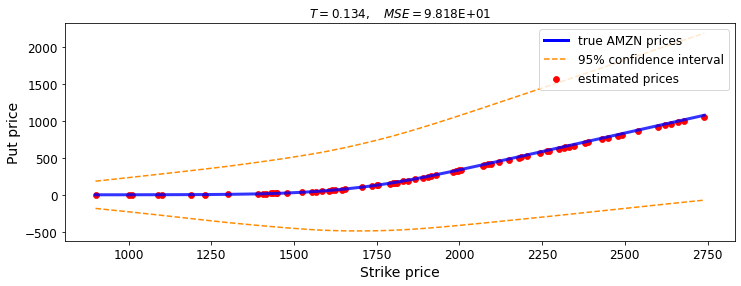
\includegraphics[width=0.9\textwidth]{real_data_amzn_put.png}
    \caption{Estimated put prices yielded by the 2-dimensional FGP model trained on real call option data.}
    \label{fig:real_data_amzn_put}
\end{figure}
\noindent Figures \ref{fig:real_data_sideview} show a sideview of the call and put price surface estimated by the model using market training data. These perhaps paint a more favorable picture of the potential of FGPs for pricing options using market data.

\begin{figure}[H]
\begin{minipage}[c]{.45\linewidth}
    \centering
    \makebox[0pt]{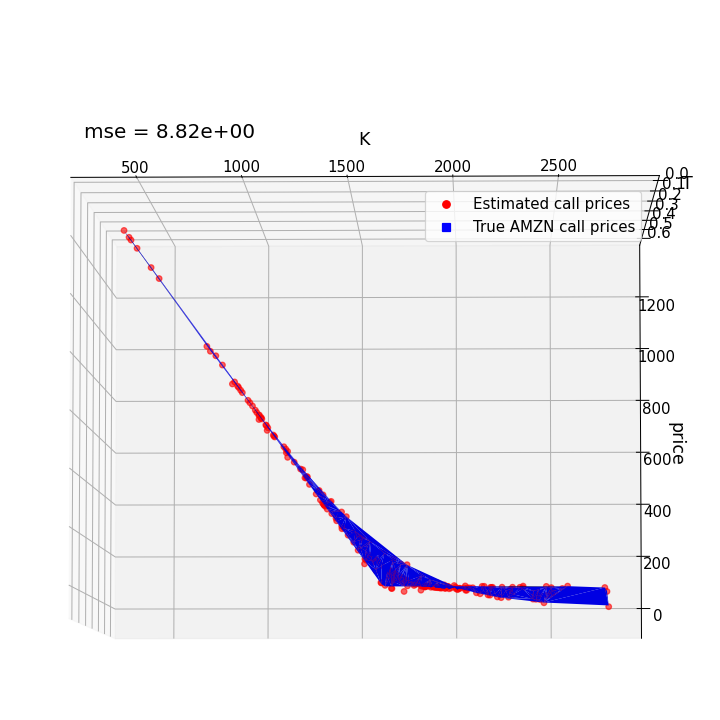
\includegraphics[width = 8.5 cm]{real_data_calls_2d_sideview_b.png}}
\end{minipage} \hfill
\begin{minipage}[c]{.45\linewidth}
    \centering
    \makebox[0pt]{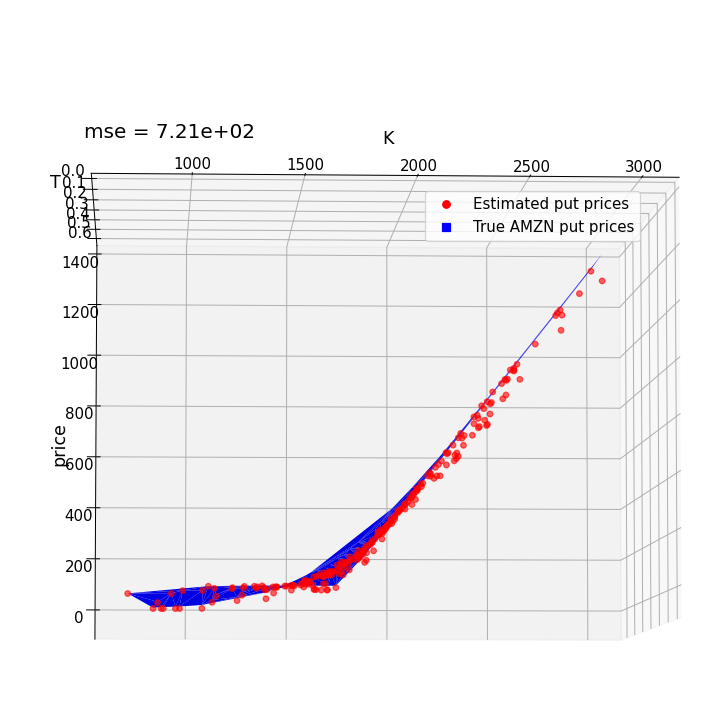
\includegraphics[width = 8.5 cm]{real_data_puts_2d_sideview_b.png}}
\end{minipage}
\caption{Sideview of estimated call price surface (left) and put price surface (right) yielded by the 2-dimensional FGP model trained on real, market call option data.}
\label{fig:real_data_sideview}
\end{figure}

\newpage
\section{Multi-output Gaussian processes}
The second part of this thesis showed how Gaussian process regression can be applied in novel situations, in particular the pricing of any European option. While this application is interesting and demonstrates the versatility of Gaussian processes, its benefit to the real world financial industry is, for the moment, purely speculative. The pricing of American and European options, however, is something of concrete use to real world finance. This third part of the thesis will thus focus on improving estimates of these option prices by using a multi-output Gaussian process. The idea here is to try to predict both option types simultaneously, and benefit from some correlation between the outputs to improve the estimates.

\subsection{Generating option prices with the binomial tree model}
Until now we have been using the Black-Scholes model to price European options. Unfortunately, this model is no longer sufficient to price American options as it doesn't allow for early exercise. Instead, we choose the binomial tree model, which can be used to price European and American options.\\
The binomial tree options pricing model was formalised in the paper ``Option pricing: A simplified approach" by Cox et al. \cite{COX1979}. The binomial tree can be seen as a discrete time approximation of the Black-Scholes model. The principle of the model is that, at each time step, the price of the underlying stock $S_0$ can either go up to a value $u S_0$ with probability $p$ or down to a value $d S_0$ with probability $1-p$. Thus, we can construct a binomial price tree of $n$ time steps that collects all the possible paths of the stock price. In fact, we define the up and down factors as: 
\begin{align*}
    u &= e^{\sigma \sqrt{T/n}} \\
    d &= e^{-\sigma \sqrt{T/n}} = 1/u
\end{align*}
where $\sigma$ is the volatility of the underlying and $T$ is the time-to-maturity. These definitions of the factors allow us to write the price at any point without building the whole pricing tree. In particular, we can write the price at the final time step $n$:
$$S_n = S_0 u^{N_u - N_d}$$
where $N_u$ is the number of times the stock went up and $N_d$ is the number of times it went down. Figure \ref{fig:binomial_tree} illustrates the binomial tree model.
\begin{figure} [H]
    \centering
    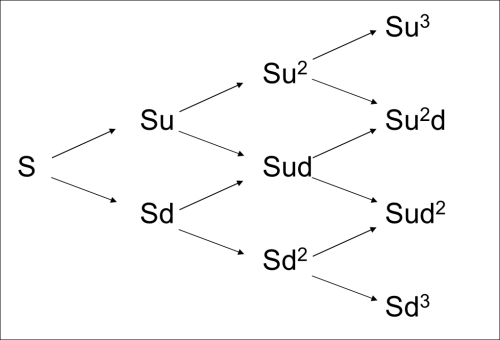
\includegraphics[width=0.5\textwidth]{binomial_tree.png}
    \caption{Illustration of the binomial tree pricing model \cite{binomialtree}.}
    \label{fig:binomial_tree}
\end{figure}
\noindent Now that we have modelised the underlying stock prices, we can turn to pricing an option on this underlying; for example we can consider a European put option of strike $K$ and time-to-maturity $T$. Under the risk neutrality assumption, the price of any option today is the discounted expectation of its future payoff. The payoff at the final time step is simply:
$$P_n = (K-S_n)_{+} = (K-S_0 u^{N_u - N_d})_{+}$$
The price at the penultimate time step can then be computed as:
$$P_{n-1} = e^{-r T/n} \left(p P_n(\text{up}) + (1-p) P_n(\text{down}) \right)$$
where $p = \frac{e^{(r-q)T/n} - d}{u - d}$, $r$ is the risk free rate and $q$ is the dividend yield. This formula means that the price at a step $t$ is the probability $p$ of the stock going up times the value of the option at time $t+\delta t$ in that case plus the probability $1-p$ of the stock going down times the value of the option at time $t+\delta t$ in that case, all discounted by the risk free rate. This formula can be applied to each time step so that the expectation of the final payoff is backpropagated to the very first time step, giving us the current price of the option.\\
In fact, the algorithm above can be modified very slightly to generate American option prices as well. At each time step, compare the binomial value $C_i$ computed using the formula above to the immediate exercise value of the option $(K-S_i)_{+}$. Whichever of the two is greater becomes the value of the option at time step $i$. Indeed, if one can exercise an option early for greater profit than the expected value of the option in the future, one should always do so.\\
One final point that should be mentioned is that in the rest of this section we will only consider put options, and not call options. The reason for this is that the price of an American call option is the same as the price for a European call option. We have actually already seen this in the proof of the No Arbitrage conditions in section \ref{sec:na_cond_proof}. Put option prices, however, differ for American and European. They can therefore be used to evaluate the performance of a multi-output model that should be able to simultaneously estimate several different, but similar, output functions.

\subsection{Gaussian processes with multiple outputs}
\subsubsection{Theory}
This section summarises concepts presented in \cite{alvarez2009} and \cite{MOGP_slides}.\\
The idea of using Gaussian process models with multiple outputs was first introduced in the field of geostatistics by Journel and Huijbregts in 1978 \cite{Journel1978}, where they are known as Linear Models of Coregionalisation (LMC). The hope behind multitask learning is that the correlation between the outputs will improve the performance of the model compared to several models learning the separate tasks independently. A simplified version of the LMC is known as the \textbf{Intrinsic Coregionalisation Model} (ICM) \cite{Goovaerts1997}, which works as follows: \\
Consider two output functions $f_1(\mathbf{x})$ and $f_2(\mathbf{x}), \ \mathbf{x} \in \mathcal{R}^p$, which we wish to approximate using a multiple output Gaussian process. Suppose we have Gaussian process $u(\mathbf{x}) \sim \text{GP}(0, k(\mathbf{x}, \mathbf{x'}))$ which we can sample twice to obtain $u^1(\mathbf{x})$ and $u^2(\mathbf{x})$. We can now approximate $f_1$ and $f_2$ by adding a scaled transformation of $u^1$ and $u^2$:
\begin{equation}
\begin{aligned}
  f_1(\mathbf{x}) &= a_1^1 u^1(\mathbf{x}) + a_1^2 u^2(\mathbf{x})\\
  f_2(\mathbf{x}) &= a_2^1 u^1(\mathbf{x}) + a_2^2 u^2(\mathbf{x})
\end{aligned}
\end{equation}
By writing $\mathbf{a^1} = [a_1^1, a_2^1]^T$, $\mathbf{a^2} = [a_1^2, a_2^2]^T$, and $\mathbf{f} = [f_1, f_2]^T$, we have:
\begin{align*}
    \text{cov}(\mathbf{f}(\mathbf{x}), \mathbf{f}(\mathbf{x'})) &= \mathbf{a}^1(\mathbf{a}^1)^T \text{cov}(u^1(\mathbf{x}), u^1(\mathbf{x'})) + \mathbf{a}^2(\mathbf{a}^2)^T \text{cov}(u^2(\mathbf{x}), u^2(\mathbf{x'})) \\
    &= \mathbf{a}^1(\mathbf{a}^1)^T k(\mathbf{x}, \mathbf{x'}) + \mathbf{a}^2(\mathbf{a}^2)^T k(\mathbf{x}, \mathbf{x'})\\
    &= [\mathbf{a}^1(\mathbf{a}^1)^T + \mathbf{a}^2(\mathbf{a}^2)^T] k(\mathbf{x}, \mathbf{x'})
\end{align*}
We define $B = \mathbf{a}^1(\mathbf{a}^1)^T + \mathbf{a}^2(\mathbf{a}^2)^T$, and obtain:
\begin{equation}
    \text{cov}(\mathbf{f}(\mathbf{x}), \mathbf{f}(\mathbf{x'})) = B k(\mathbf{x}, \mathbf{x'}) = 
    \begin{pmatrix}
        b_{11} & b_{12}\\
        b_{21} & b_{22}
    \end{pmatrix} k(\mathbf{x}, \mathbf{x'})
\end{equation}
In fact, using the Kronecker product $\otimes$, we can write:
\begin{equation}
    \begin{bmatrix}
        \mathbf{f}_1\\
        \mathbf{f}_2
    \end{bmatrix} = 
    \begin{bmatrix}
        f_1(\mathbf{x}_1)\\
        \vdots \\
        f_1(\mathbf{x}_N)\\
        f_2(\mathbf{x}_1)\\
        \vdots \\
        f_2(\mathbf{x}_N)\\
    \end{bmatrix} \sim \mathcal{N}\left(
    \begin{bmatrix}
        \mathbf{0}^N\\
        \mathbf{0}^N
    \end{bmatrix}, B \otimes K \right)
\end{equation}
If $B$ is a $(2 \times 2)$ matrix and $K$ is a $(N \times N)$ matrix, then $B \otimes K$ is a $(2N \times 2N)$ matrix.\\
We can generalise this model to account for any number of tasks. Consider a set of functions $\{f_d(\mathbf{x})\}_{d = 1}^D$. In the ICM, we have
\begin{equation}
    f_d(\mathbf{x}) = \sum_{i = 1}^{R} a_d^i u^i(\mathbf{x}) 
\end{equation}
where the $u^i$ are GPs sampled independently from $u \sim \mathcal{N}(0, k(\mathbf{x}, \mathbf{x'}))$.\\
With $\mathbf{f} = [f_1, f_2, \dots, f_D]^T$ and $A = [\mathbf{a}^1, \mathbf{a}^2, \dots, \mathbf{a}^R]$, we have
\begin{equation}
    \text{cov}(\mathbf{f}(\mathbf{x}), \mathbf{f}(\mathbf{x'})) = AA^T k(\mathbf{x}, \mathbf{x'}) = B k(\mathbf{x}, \mathbf{x'})
\end{equation}
\newline
In 2005, Teh et al. \cite{Teh2005} propose a slightly different model, called the \textbf{Semiparametric Latent Factor Model} (SLFM). In this model, instead of using $R$ samples $u^i(\mathbf{x})$ with the same covariance function $k(\mathbf{x}, \mathbf{x'})$, they use $Q$ samples from $u_q(\mathbf{x})$ processes with different covariance functions:
\begin{equation}
\begin{aligned}
  f_1(\mathbf{x}) &= a_{1,1} u_1(\mathbf{x}) + a_{1,2} u_2(\mathbf{x})\\
  f_2(\mathbf{x}) &= a_{2,1} u_1(\mathbf{x}) + a_{2,2} u_2(\mathbf{x})
\end{aligned}
\end{equation}
With $\mathbf{a}_1 = [a_{1,1}, a_{2,1}]^T$ and $\mathbf{a}_2 = [a_{1,2}, a_{2,2}]^T$, we get:
\begin{equation}
    \text{cov}(\mathbf{f}(\mathbf{x}), \mathbf{f}(\mathbf{x'})) = \mathbf{a}_1 (\mathbf{a}_1)^T k_1(\mathbf{x}, \mathbf{x'}) + \mathbf{a}_2 (\mathbf{a}_2)^T k_2(\mathbf{x}, \mathbf{x'}) = B_1 k_1(\mathbf{x}, \mathbf{x'}) + B_2 k_2(\mathbf{x}, \mathbf{x'})
\end{equation}
In the generalised form, the SLFM model is written:
\begin{equation}
\begin{aligned}
  f_d(\mathbf{x}) &= \sum_{q = 1}^{Q} a_{d,q} u_q(\mathbf{x}) \\
  \text{cov}(\mathbf{f}(\mathbf{x}), \mathbf{f}(\mathbf{x'})) &= \sum_{q = 1}^Q \mathbf{a}_q (\mathbf{a}_q)^T k_q(\mathbf{x}, \mathbf{x'}) = \sum_{q = 1}^Q B_q k_q(\mathbf{x}, \mathbf{x'})
\end{aligned}
\end{equation}
\newline
The \textbf{Linear Model of Coregionalisation} can be seen as a generalisation of the ICM and the SLFM, allowing several independent samples from GPs with different covariances.
\begin{equation}
\label{LMC_eq}
\begin{aligned}
  f_d(\mathbf{x}) &= \sum_{q = 1}^{Q} \sum_{i = 1}^{R_q} a^i_{d,q} u^i_q(\mathbf{x}) \\
  \text{cov}(\mathbf{f}(\mathbf{x}), \mathbf{f}(\mathbf{x'})) &= \sum_{q = 1}^Q A_q (A_q)^T k_q(\mathbf{x}, \mathbf{x'}) = \sum_{q = 1}^Q B_q k_q(\mathbf{x}, \mathbf{x'})
\end{aligned}
\end{equation}
where $A_q = [\mathbf{a}^1_q, \mathbf{a}^2_q, \dots, \mathbf{a}^{R_q}_q]$.\\
The $B_q$ are known as coregionalisation matrices; they have size $(D \times D)$.
In Kronecker product notation, we have:
\begin{equation}
    \begin{bmatrix}
        \mathbf{f}_1\\
        \vdots\\
        \mathbf{f}_D
    \end{bmatrix} = 
    \begin{bmatrix}
        f_1(\mathbf{x}_1)\\
        \vdots \\
        f_1(\mathbf{x}_N)\\
        \vdots \\
        f_D(\mathbf{x}_1)\\
        \vdots \\
        f_D(\mathbf{x}_N)\\
    \end{bmatrix} \sim \mathcal{N}\left(
    \begin{bmatrix}
        \mathbf{0}^N\\
        \vdots \\
        \mathbf{0}^N
    \end{bmatrix}, \sum_{q = 1}^Q B_q \otimes K_q \right)
\end{equation}
\newline
The LMC is actually a somewhat restrictive way to construct multiple output Gaussian processes, since it involves the instantaneous mixing of independent processes. In 2002, Higdon \cite{Higdon2002} generalised it further by convolving a base process $u(\mathbf{x})$ with a smoothing kernel $G_d(\mathbf{x})$. This is called a \textbf{Convolution Process}.
\begin{equation}
    f_d(\mathbf{x}) = \int_\mathcal{X} G_d(\mathbf{x} - \mathbf{z}) u(\mathbf{z}) d\mathbf{z}
\end{equation}
More generally, we can include more latent processes $u_1(\mathbf{x}), u_2(\mathbf{x}), \dots, u_Q(\mathbf{x})$:
\begin{equation}
\label{convolution_process_eq}
\begin{aligned}
  f_d(\mathbf{x}) &= \sum_{q = 1}^{Q} \sum_{i = 1}^{R_q} \int_\mathcal{X} G^i_{d,q}(\mathbf{x} - \mathbf{z}) u^i_q(\mathbf{z}) d\mathbf{z} \\
  \text{cov}(f_d(\mathbf{x}), f_{d'}(\mathbf{x'})) &= \sum_{q = 1}^Q \sum_{i = 1}^{R_q} \int_\mathcal{X} G^i_{d,q}(\mathbf{x} - \mathbf{z}) \int_\mathcal{X} G^i_{d',q}(\mathbf{x'} - \mathbf{z'}) k_q(\mathbf{z}, \mathbf{z'}) d\mathbf{z'} d\mathbf{z}
\end{aligned}
\end{equation}
Note that if we define the smoothing kernel as $G^i_{d,q}(\mathbf{x} - \mathbf{z}) = a^i_{d,q} \delta(\mathbf{x} - \mathbf{z})$ the integrals in equation \ref{convolution_process_eq} are easily solved and yield the same expressions as in equation \ref{LMC_eq}. Thus we see that the LMC is just a particular case of a convolution process, and we also see that the Dirac delta function matches the instantaneous mixing we introduced to describe the LMC.

\subsubsection{\texttt{GPyTorch} implementation}
There are many implementations of Multiple Output Gaussian Processes in Python, of which the following were explored: \texttt{MOGPTK} \cite{mogptk}, \texttt{GPflow} \cite{GPflow2017}, and \texttt{GPyTorch} \cite{gardner2018gpytorch}. The first implementation, \texttt{MOGPTK}, is the only one of the three to implement a convolution process (rather than just an LMC). It also implements a method for setting appropriate initial conditions on the hyperparameters. In this sense it is much more advanced than either of the other two implementations. Unfortunately, it does not yet support having multidimensional inputs which makes it unusable for pricing options using both strike and time-to-maturity. Nevertheless, if the package is updated in the future to include this functionality it would be interesting to revisit it. The second implementation, \texttt{GPflow}, does allow for multiple input dimensions, but only implements an LMC. Additionally, as we'll see later, the advantages of using a multi-output Gaussian process are limited when we consider noiseless data. It can however be interesting to consider different sets of training data for each task, as this would open another avenue for co-learning. This last functionality, of splitting the input data for each output, is only available on \texttt{GPyTorch}, and so this is the package we'll be using.\\
The \texttt{GPyTorch} package bases its implementation of multi-task Gaussian processes on the paper by Bonilla et al. \cite{Bonilla2007}. The paper describes an intrinsic coregionalisation model as: 
\begin{equation}
\label{Bonilla_eq}
\text{cov}(f_d(\mathbf{x}), f_{d'}(\mathbf{x'})) = K^f \otimes k^x(\mathbf{x}, \mathbf{x'})
\end{equation}
where $K^f$ is a positive semi-definite matrix that specifies the inter-task similarities. The paper then introduces several approximations to speed up computations; in particular they parametrise the $K^f$ matrix using a Probabilistic Principal Component Analysis (PPCA) model \cite{Tipping1999}.\\
Given the expression in equation \ref{Bonilla_eq}, the posterior mean prediction of the model at a test point $\mathbf{x_*}$ is given by:
\begin{equation}
    \mathbf{f_*}(\mathbf{x_*}) = (K^f \otimes \mathbf{k_*}^x)^T \Lambda^{-1} \mathbf{y}, \qquad \Lambda = K^f \otimes K^x + \Sigma \otimes I
\end{equation}
where $\mathbf{k_*}^x$ is the vector of covariances between the test point $\mathbf{x_*}$ and all the training points, $K^x$ is the matrix of covariances between training points, and $\Sigma$ is a $(D \times D)$ matrix in which the $(d,d)^\text{th}$ element is the observation noise variance $\sigma_d^2$. Note that this is a heteroskedastic model where each output task has a separate noise term.\\
The paper presents a proof that, under the assumption of noiseless observations, predictions using the ICM with an identical data set for each output are equivalent to independent predictions over each output. This is why using the \texttt{GPflow} implementation would have yielded poor results. Since the proof is succinct and of interest, we reproduce it here:
\begin{proof}
In the noiseless case $\Sigma = 0$, and so we have:
\begin{align*}
    \mathbf{f_*}(\mathbf{x_*}) &= (K^f \otimes \mathbf{k_*}^x)^T (K^f \otimes K^x)^{-1} \mathbf{y}\\
    &= ((K^f)^T \otimes (\mathbf{k_*}^x)^T) ((K^f)^{-1} \otimes (K^x)^{-1}) \mathbf{y}\\
    &= [(K^f)^T (K^f)^{-1} \otimes (\mathbf{k_*}^x)^T (K^x)^{-1}] \mathbf{y}\\
    &= \begin{pmatrix}
        (\mathbf{k_*}^x)^T (K^x)^{-1} \mathbf{y}_1\\
        \vdots\\
        (\mathbf{k_*}^x)^T (K^x)^{-1} \mathbf{y}_D
    \end{pmatrix}
\end{align*}
Thus, in the noiseless case, the predictions for a task $d$ depend only on the targets $\mathbf{y}_d$. In other words, there is no inter-task transfer.
\end{proof}
\noindent To illustrate this point, in figures \ref{fig:mogp_indep_training} and \ref{fig:mogp_same_inputs} we plot the predictions of two Gaussian processes trained separately on American and European put data and compare the obtained mean squared error to when we use an ICM as described above. The data is generated using the binomial tree model with $n = 100$. As such, there is very little observation noise. In figure \ref{fig:mogp_indep_training}, we define two Gaussian processes with constant mean function and an RBF kernel, and we train them separately on a grid of 100 $(T, K)$ training points of American put data and European put data. In figure \ref{fig:mogp_same_inputs}, we define a single multi-task ICM with constant mean function and where $k^x(\mathbf{x}, \mathbf{x'})$ is an RBF kernel. The $K^f$ matrix is learnt as a hyperparameter (or 4 hyperparameters in the two dimensional output case). The ICM model is trained on the same grid of 100 $(T, K)$ training points, with the output $\mathbf{y}$ being a concatenation of the American put prices and the European put prices. Clearly the figures show that the two independent Gaussian processes yield far better predictions, thus showing the limitations of the IMC in the noiseless (or quasi-noiseless) case. It should be noted that the reason the IMC predictions aren't equivalent to the independent predictions is because the IMC has only one RBF kernel and must tune its hyperparameters to fit both American and European puts at the same time, whereas the independent models each have their own separate RBF kernels and can thus tune the hyperparameters to fit only American puts or only European puts.

\begin{figure}[H]
\begin{minipage}[c]{.9\linewidth}
    \centering
    \makebox[0pt]{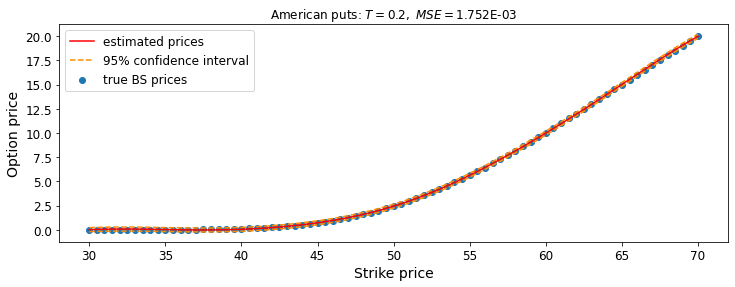
\includegraphics[width = 12 cm]{mogp_indep_training_am_puts.png}}
\end{minipage} \vfill
\begin{minipage}[c]{.9\linewidth}
    \centering
    \makebox[0pt]{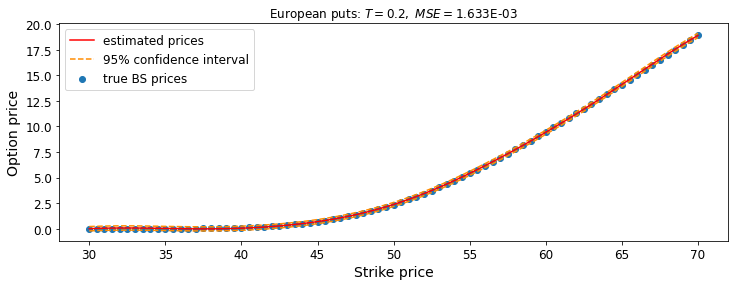
\includegraphics[width = 12 cm]{mogp_indep_training_eur_puts.png}}
\end{minipage}
\caption{Estimated prices for American puts (top) and European puts (bottom) yielded by two independent Gaussian processes, trained on a grid of 100 $(T, K)$ points.}
\label{fig:mogp_indep_training}
\end{figure}

\begin{figure}[H]
\begin{minipage}[c]{.9\linewidth}
    \centering
    \makebox[0pt]{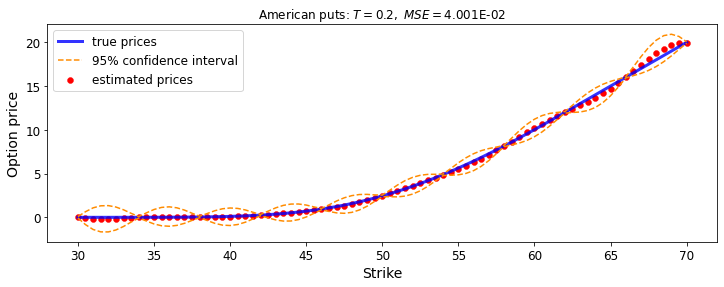
\includegraphics[width = 12 cm]{mogp_same_inputs_am_puts.png}}
\end{minipage} \vfill
\begin{minipage}[c]{.9\linewidth}
    \centering
    \makebox[0pt]{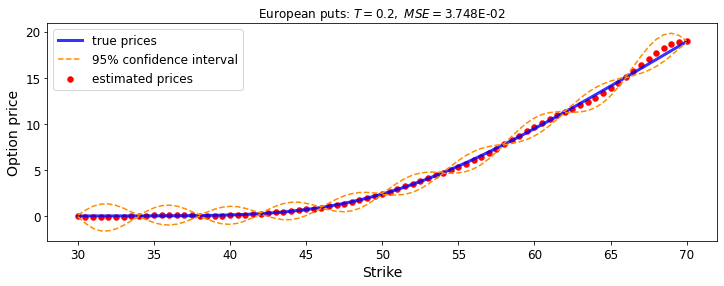
\includegraphics[width = 12 cm]{mogp_same_inputs_eur_puts.png}}
\end{minipage}
\caption{Estimated prices for American puts (top) and European puts (bottom) yielded by a single multi-task Gaussian process, trained on a grid of 100 $(T, K)$ points.}
\label{fig:mogp_same_inputs}
\end{figure}
\noindent In order to justify the use of a multi-output Gaussian process, we must therefore either use very noisy data, or we can try to implement a model that uses different input data for each output function. The intuition is that, if we train the model using a grid of 100 $(T, K)$ points associated to American puts and a separate grid of 100 $(T', K')$ points associated to European puts, then the model might learn something about American puts at the $(T', K')$ points and likewise for European puts at the $(T, K)$ points. In fact, if we choose the $(T', K')$ grid to be shifted by half a step w.r.t. the $(T, K)$ grid, then perhaps the model can reduce its uncertainty in the place where the uncertainty should be highest (halfway between each $(T, K)$ point).\\
\texttt{GPyTorch} implements this disparate input model by replacing the Kronecker product in the previous formulae with a Hadamard product $\odot$. The Hadamard product is an element-wise matrix multiplication between two matrices of identical size. As such, the $K^f$ matrix must also be modified. The package chooses to add an additional index input parameter, and to replace $K^f$ with an index kernel 
\begin{equation}
    k^\text{index}(i, j) = K^f_{i,j}
\end{equation}
There are as many possible indices as there are tasks, meaning $D$ of them. We want the full matrix of index covariances between $N$ training points $\mathbf{x}$ to be of size $(N \times N)$, whereas $K^f$ is only of size $(D \times D)$. We can split the training data evenly into $D$ batches of $N/D$ training points $(\mathbf{x}_m^i, i)$, $m \in [1, \dots, N/D]$, $i \in [1, \dots, D]$. Note that the points $\mathbf{x}_m^i$ can differ between index batches, meaning that we can associate a different grid of inputs to the different tasks. The index kernel associated to one batch of $N/D$ points becomes
\begin{equation}
    K^{\text{index}, N/D}_{i,j} = 
    \begin{pmatrix}
        K^\text{index}_{i,j} & \dots & K^\text{index}_{i,j} \\
        \vdots & \ddots & \vdots \\
        K^\text{index}_{i,j} & \dots & K^\text{index}_{i,j}
    \end{pmatrix}
\end{equation}
That is to say that it becomes a block of identical values of size $(N/D \times N/D)$. The full index kernel associated to all the training points becomes
\begin{equation}
    K^\text{index} = \begin{pmatrix}
        K^{\text{index}, N/D}_{1,1} & \dots & K^{\text{index}, N/D}_{1,D} \\
        \vdots & \ddots & \vdots \\
        K^{\text{index}, N/D}_{D,1} & \dots & K^{\text{index}, N/D}_{D,D}
    \end{pmatrix}
\end{equation}
That is to say it becomes a block matrix containing $D \times D$ blocks of size $(N/D \times N/D)$. So the size of the full matrix is $(N \times N)$, which is what we wanted. The posterior mean now takes the form
\begin{equation}
    \mathbf{f_*}((\mathbf{x_*}, i)) = (K^\text{index}_i \odot \mathbf{k_*}^x)^T \Lambda^{-1} \mathbf{y}, \qquad \Lambda = K^\text{index} \odot K^x + \Sigma
\end{equation}
where $K^\text{index}_i = [K^{\text{index}, N/D}_{i,1}, K^{\text{index}, N/D}_{i,2}, \dots, K^{\text{index}, N/D}_{i,D}]^T$. It should also be noted that in the paper by Bonilla et al. \cite{Bonilla2007}, the $\Sigma$ matrix was of the heteroskedastic form
$$
    \Sigma = 
    \begin{pmatrix}
        \sigma_1^2 & \dots & 0 \\
        \vdots & \ddots & \vdots\\
        0 & \dots & \sigma_D^2
    \end{pmatrix}
$$
Unfortunately, the Hadamard multi-task GP implementation in \texttt{GPyTorch} does not yet support heteroskedacity. As such, the $\Sigma$ matrix is here of the form $\sigma_\epsilon^2 I^{N\times N}$.
\begin{figure}[H]
\begin{minipage}[c]{.9\linewidth}
    \centering
    \makebox[0pt]{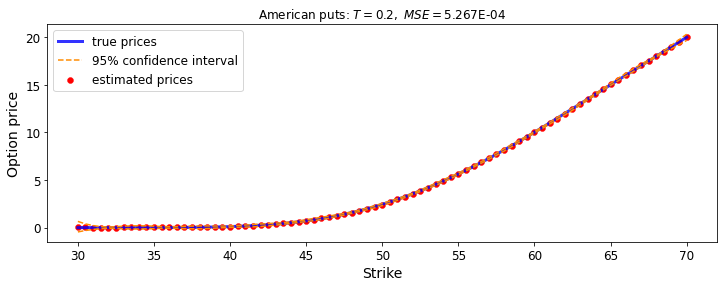
\includegraphics[width = 12 cm]{mogp_diff_inputs_am_puts.png}}
\end{minipage} \vfill
\begin{minipage}[c]{.9\linewidth}
    \centering
    \makebox[0pt]{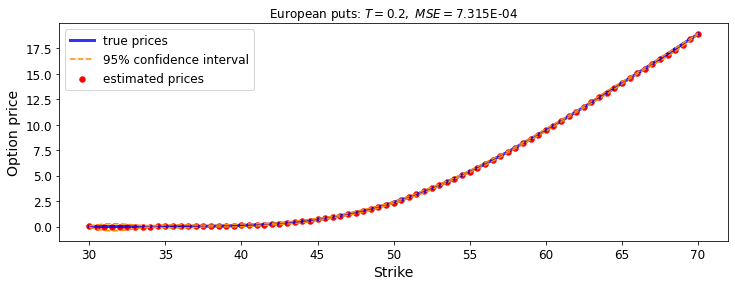
\includegraphics[width = 12 cm]{mogp_diff_inputs_eur_puts.png}}
\end{minipage}
\caption{Estimated prices for American puts (top) and European puts (bottom) yielded by a single Hadamard multi-task Gaussian process, trained on a grid of 100 $(T, K)$ points for the American puts and a separate grid of 100 $(T', K')$ points for the European puts. The $(T', K')$ points are shifted to be halfway between the $(T, K)$ points, where the uncertainty of the model should be greatest.}
\label{fig:mogp_diff_inputs}
\end{figure}
\noindent In figure \ref{fig:mogp_diff_inputs} we illustrate the performance of this Hadamard model. Here we once again use data generated by the binomial tree model. However, whereas in figures \ref{fig:mogp_indep_training} and \ref{fig:mogp_same_inputs} we used the same grid of 100 $(T, K)$ points as inputs for the American put task and the European put task, in figure \ref{fig:mogp_diff_inputs} we use separate grids of 100 $(T, K)$ points for the American put task and 100 shifted $(T', K')$ points for the European put task. The result is a much lower mean squared error than in the previous multi-task model, using the Kronecker delta, and even a lower mean squared error than the two independently trained Gaussian processes. Recall as well that the two independent models can tune their hyperparameters to fit their specific task, whereas the Hadamard multi-task model must tune its hyperparameters to fit both tasks simultaneously, which makes it that much more impressive that the Hadamard model can perform so well.


\subsubsection{Note about \texttt{GPyTorch}}
A major flaw of the \texttt{GPyTorch} implementation is that there seems to be an error in the way it does the Cholesky decomposition necessary to invert the $\Lambda$ matrix. Indeed, often the training process of the model will raise the exception that the Cholesky decomposition is not possible due to the matrix not being positive semi-definite (actually it might even require that the matrix be positive definite, as is the case with many other packages). This is most likely due to the gradient descent method finding hyperparameters that render the $\Lambda$ matrix non positive definite. In theory this should not really be possible if the kernels have been properly defined to be positive definite, which is why there is likely a code error somewhere in the package.\\
One possible solution is to ensure the noise parameter $\sigma_\epsilon$ does not become too small, but the package actually already constrains it to be greater than $10^{-4}$. We can manually change the constraint to higher values but we wouldn't want the noise parameter to be unnecessarily high either.\\
Lowering the learning rate of the optimiser also seems to mitigate this error, but that is also not an ideal solution since it greatly increases the time required for training and limits the learning potential of the model.\\
Another solution would be to check whether a new set of hyperparameters breaks the Cholesky decomposition before adopting it, and forcing the optimiser to choose a new set if the former doesn't work. However, it is not certain that the hyperparameters that minimise the negative log likelihood are also valid for the Cholesky decomposition, and so this modified algorithm might never have an end.\\
A last, inelegant but easy, solution to the problem is simply to keep running the training algorithm till it works. Indeed, every so often the optimiser avoids all hyperparameter sets that break the decomposition and so yields a trained, working model. There is, of course, no guarantee of how many training attempts this could take.\\
It also goes without saying that the best (and most time-consuming) solution would be to forego the use of the \texttt{GPyTorch} package and re-write the model from scratch (hopefully without errors this time).

\newpage
\section{Other works and possible extensions}
This section explores a few extensions or improvements that could be made upon the work previously presented. A brief summary of the theory behind more recent advances in Gaussian process regression is given, as a potential starting point for further research.

\subsection{Inducing variables and sparse variational GPs}
One problem that we haven't yet discussed in this thesis, but which is nevertheless noteworthy, is the computational complexity of the GP regression algorithm. Indeed, if $n$ is the number of inputs in our training set, the algorithm's complexity scales as $O(n^3)$. This is because it requires the inversion of the covariance matrix of training points $K^{n \times n}$. This complexity means that using large datasets is intractable. So far we have not really encountered the issue, but it is easy to imagine a scenario where we might want three or more input variables to our model, rather than the usual two $(T, K)$. In such a case, if we keep approximately ten inputs per dimension, instead of having 100 training points, we'll have 1000 or more. In fact, such a scenario was implemented in the thesis by Daniel Montagna \cite{Montagna2021}, where he considers a GP taking as input not only time-to-maturity and strike, but also the price of a variance swap. Thus, it would be interesting to have a way of reducing the complexity of the algorithm.\\
One solution that has been explored is the use of inducing variables. The idea is to choose a new smaller set of $m$ training variables (rather than $n$), and reduce the complexity from $O(n^3)$ to $O(n m^2)$. The inducing variables can be seen as a compression of the real observations. GPs built using inducing variables are called `sparse' since they use fewer training points.\\
The reduction in complexity comes from the fact that we can replace the covariance matrix $K^{n \times n}$ by an approximation of the form $Q^{n \times n} = K^{n \times m} K^{m \times m} K^{m\times n}$. Note that this is just one example of an approximation called the projected process (PP) approximation \cite{Seeger2003}; others, such as the sparse pseudo-input GP (SPGP) method \cite{Snelson2006} are also possible.\\
The only issue that remains is how to choose the inducing points. Suppose $f$ is the function we wish to approximate, $\mathbf{f}$ a vector of original function points, and $\mathbf{y} = \mathbf{f} + \boldsymbol{\epsilon}$ our noisy observations. The only condition on the choice of inducing points $\mathbf{u}$ is that they must be jointly Gaussian distributed with $\mathbf{f}$:
\begin{equation}
    \begin{pmatrix}
        \mathbf{f}\\
        \mathbf{u}
    \end{pmatrix} = \mathcal{N}(\mathbf{0}, \mathbf{K})
\end{equation}
Often $\mathbf{u}$ is chosen from the same domain as $\mathbf{f}$ itself, but it is also possible to choose a linear transformation of $\mathbf{f}$, such as its gradient in select points. In reality, the choice of the inducing points $\mathbf{u}$ is not so trivial, since it must minimise the information loss from $\mathbf{y}$ to $\mathbf{u}$ as much as possible. One innovation was introduced by Titsias in 2009 \cite{Titsias09}. He proposed a variational approach to learning the inducing points. He found that the conditional density of the data given the inducing points could written as:
\begin{equation}
\label{eq:variational_bound}
\begin{aligned}
    \log{p(\mathbf{y} | \mathbf{u})} &= \log{\int p(\mathbf{y} | \mathbf{f}) p(\mathbf{f} | \mathbf{u}) d\mathbf{f}}\\
        &= \int p(\mathbf{f} | \mathbf{u}) \log{p(\mathbf{y} | \mathbf{f})} d\mathbf{f} + \text{KL}(p(\mathbf{f}|\mathbf{u}, \mathbf{y})\ \| \ p(\mathbf{f}|\mathbf{u}))
\end{aligned}
\end{equation}
where KL$(\cdot, \cdot)$ is the Kullback-Leibler divergence, defined as:
\begin{equation}
    \text{KL}(p(\mathbf{f}|\mathbf{u}, \mathbf{y})\ \| \ p(\mathbf{f}|\mathbf{u})) = \int p(\mathbf{f}|\mathbf{u}) \log{\frac{p(\mathbf{f}|\mathbf{u})}{p(\mathbf{f}|\mathbf{u}, \mathbf{y})}} d\mathbf{u}
\end{equation}
His idea was to find the $\mathbf{u}$ that minimises the Kullback-Leibler divergence between the true density $p(\mathbf{f}|\mathbf{u}, \mathbf{y})$ and the approximating density $p(\mathbf{f}|\mathbf{u})$, using equation \ref{eq:variational_bound}. Minimising this quantity amounts to finding the optimal compression of $\mathbf{y}$ to $\mathbf{u}$.

\subsection{Deep GPs}
Another somewhat recent innovation in GP modelling is the use of deep Gaussian processes, introduced by Damianou and Lawrence in 2013 \cite{damianou2013}. Their idea is quite simple, though its implementation is less so. Instead of approximating the function $f$ by a single Gaussian process, they rather model it as a successive chain of Gaussian processes, where the output of the first becomes the input of the second and the output of the second becomes the input of the third, and so on... A simple illustration is given in figure \ref{fig:deep_gp}. 
\begin{figure}[H]
\begin{center}
\begin{minipage}[r]{.24\linewidth}
    \centering
    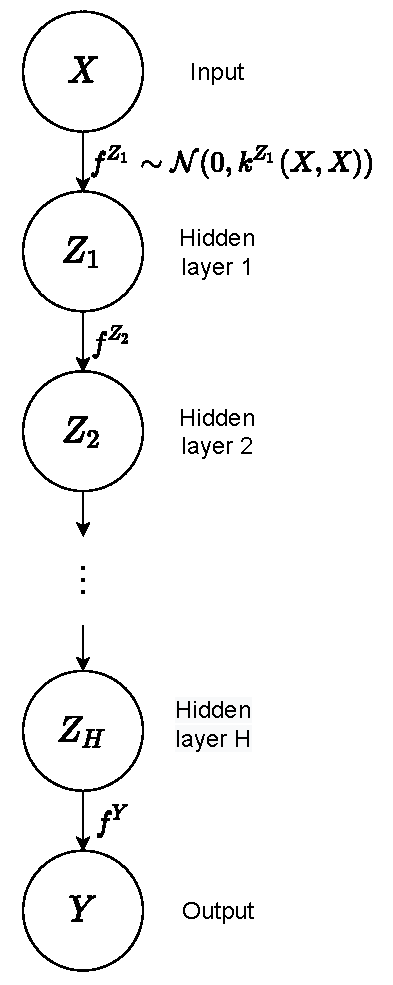
\includegraphics[width = \linewidth]{deep_gp.pdf}
\end{minipage}
\begin{minipage}[l]{.4\linewidth}
    \centering
    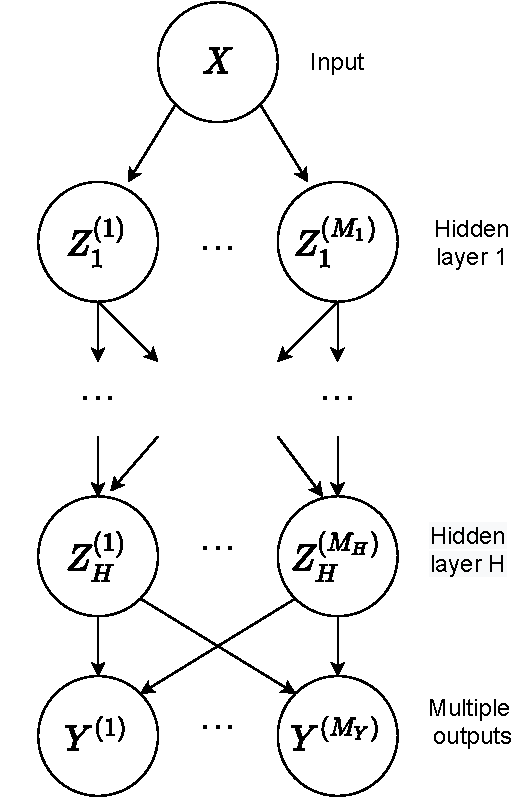
\includegraphics[width = \linewidth]{deep_mogp.pdf}
\end{minipage}
\caption{Simple illustration of a chain of Gaussian processes forming a deep GP (left), and illustration of the horizontal extension of this deep GP to include multiple outputs at each layer (right).}
\label{fig:deep_gp}
\end{center}
\end{figure}
\noindent This structure is very similar to that of a neural network. In fact, in their paper, Damianou and Lawrence even label the successive input/output variables as `layers'. Let us illustrate a simple example, with one hidden layer $Z$.\\
As before, we wish to approximate the function $f$ and we have noisy observations $\mathbf{y} = f(\mathbf{x}) + \boldsymbol{\epsilon}$. We now write:
\begin{equation}
    \begin{aligned}
        \mathbf{z} &= f^Z(\mathbf{x}) + \boldsymbol{\epsilon}^Z\\
        \mathbf{y} &= f^Y(\mathbf{z}) + \boldsymbol{\epsilon}^Y
    \end{aligned}
\end{equation}
Here we make the assumption that $f^Z$ and $f^Y$ are two independent Gaussian processes $f^Z \sim \mathcal{N}(\mathbf{0}, k^Z(\mathbf{X}, \mathbf{X}))$ and $f^Y \sim \mathcal{N}(\mathbf{0}, k^Y(\mathbf{Z}, \mathbf{Z}))$.\\
While the idea behind deep GPs is simple, a complication arises when we consider how to train such a model. Indeed, Damianou and Lawrence underline that Bayesian training requires the computation of the density:
\begin{equation}
    \log{p(\mathbf{Y})} = \int_{\mathbf{X}, \mathbf{Z}} p(\mathbf{Y}|\mathbf{Z}) p(\mathbf{Z}|\mathbf{X})p(\mathbf{X})
 \end{equation}
However, this integral is intractable due to the nonlinear way in which $X$ and $Z$ are treated through the GP priors $f^Y$ and $f^Z$. Their solution to this problem is actually the same as the one from the previous section: they introduce inducing points and create a variational lower bound on $\log{p(\mathbf{Y})}$. This lower bound once again contains a Kullback-Leibler term.\\
One final point of interest to note is that Damianou and Lawrence explore how the structure of figure \ref{fig:deep_gp} can be extended horizontally. They note that such a horizontal hierarchy could be seen as a multiple output Gaussian process. Deep Gaussian processes then appear as a natural extension of the multi-task GPs that we've already explored in this thesis. 


\subsection{Fully Bayesian hyperparameter learning}
Another extension to consider is the possibility of using a fully Bayesian method to learn the hyperparameter values. In this thesis, since we used Maximum Likelihood Estimation, we obtained a posterior distribution $p(\mathbf{y}^*|\mathbf{y}, \boldsymbol{\beta})$ conditioned not only on the observation data $\mathbf{y}$, but also on the hyperparameters $\boldsymbol{\beta}$. In reality, the distribution a fully Bayesian method would yield is simply conditioned on the data: $p(\mathbf{y}^*|\mathbf{y})$. This doesn't completely invalidate the MLE method; it can still be seen as a heuristic method that behaves approximately as you would expect (for example, the confidence bounds narrow down close to noiseless observations and widen far away from observed training data points). In addition, when the number of hyperparameters is small next to the training set size, the MLE solution should be fairly close to the true Bayesian solution.\\
However, while the MLE method is a reasonable approximation, it would still be interesting to compute a correct Bayesian posterior distribution. This has actually already been done in 2019 by Tegner and Roberts \cite{tegner2019}. I reproduce here a simplified version of their approach (originally explained in \cite{GPpredictioninterval}).\\
They first choose prior distributions $p(\boldsymbol{\beta})$ over the hyperparameters and expand the posterior distribution as:
\begin{equation}
    p(\mathbf{y}^*|\mathbf{y}) = \int_{\boldsymbol{\beta}} p(\mathbf{y}^*, \boldsymbol{\beta}|\mathbf{y}) = \int_{\boldsymbol{\beta}} p(\mathbf{y}^*| \boldsymbol{\beta}, \mathbf{y}) p(\boldsymbol{\beta}| \mathbf{y})
\end{equation}
Unfortunately, this integral is not tractable. To get around this problem, they use a Markov Chain Monte Carlo method to represent the posterior with samples. More specifically, they use elliptical slice sampling to draw samples $\hat{\boldsymbol{\beta}}$ from $p(\boldsymbol{\beta}| \mathbf{y})$, and then use these hyperparameter samples to obtain observation samples $\hat{\mathbf{y}}^*$ from $p(\mathbf{y}^*| \hat{\boldsymbol{\beta}}, \mathbf{y})$. They can then construct the desired posterior distribution from the $\hat{\mathbf{y}}^*$ samples. Since this method does not keep the hyperparameters fixed during the sampling of the posterior distribution, it is able to take into account some of the uncertainty caused by the lack of knowledge about the hyperparameters. This was not the case in the MLE method.

\newpage
\section{Conclusion}
In this thesis, we've established a fundamental understanding of Gaussian process regression. We've also shown how to implement such an algorithm in Python, and the challenges that come with such an implementation. Notably, we greatly improved our estimates on Greeks (specifically Delta) by setting boundaries on the values of the length scale hyperparameters, and more importantly by using a quasi-random data set rather than an equally-spaced data set. We were also able to build on the work of Ludkovski and Saporito \cite{Ludkovski2020} by implementing an automatic differentiation feature into our Greek estimation model, allowing greater flexibility in the potential computation of different Greeks in the future.\\
In a second part, we implemented a functional Gaussian process that can price any European payoff function, and compared it to the finite elements method which was our reference point. We noted that the FGP model usually performed slightly better than the FEM, and sometimes performed much better (as in the case of a discontinuous payoff function). Unfortunately, the FGP model showed limitations in its ability to extrapolate, which the FEM is also unable to do. The FGP model also performed significantly worse when it was trained and tested on market data, rather than Black-Scholes prices.  In this sense, this first extension on GP regression was a partial success; the FGP model performed better than the reference point in the first test cases, but still showed some limitations when applied to more challenging scenarios.\\
Alongside the implementation of the FGP, we explored the application of the No Arbitrage conditions. We found that using rejection sampling to generate valid samples was not feasible, and instead chose to project the initial, non-valid samples onto the closest price curve that satisfies the conditions. When the conditions were implemented in two dimensions ($T$ and $K$), we noticed that the mean squared error on the estimated price surface was halved after the projection (meaning after the conditions were applied). This is very satisfying, as it implies that projected prices that satisfy the conditions are more accurate than the initial, sampled prices that didn't.\\
A final extension covered by this thesis explored the use of a multi-output Gaussian process to improve estimates on the prices of both American and European puts. Here, we once again underlined the limitations of such a model, in particular that, when considering noiseless data, using the same input data set for each output function yields no inter-task transfer. Indeed, in order to take advantage of the correlations between American and European prices, we had to design a model that could take a grid of $(T, K)$ points as input for the first output (American option prices) and a different, shifted grid of $(T', K')$ inputs for the second output (European option prices). We then showed that, using a model with different input sets for each output, the multi-output GP performed better than when using two independent GP models, trained separately on European and American data. Specifically, the mean squared error on the prices yielded by the multi-output GP model was one order of magnitude smaller than for the two independent models.\\
Overall, we have thus shown the versatility of Gaussian process regression, having applied it to two novel scenarios. In the first, we modified the input space to create a very general model that can price any European option. In the second, we modified the output space in order to combine two models for pricing American and European options into one model that is greater than the sum of its parts. We ended by presenting a few more potential extensions or improvements that have been discussed in other works from the last decade, and that could become the basis of promising innovations in the future.


\newpage

\bibliographystyle{ieeetr}
\bibliography{ref} % Entries are in the "ref.bib" file

\newpage

\appendix

\includepdf[pages=-]{declaration_of_originality.pdf}
\end{document}
